\documentclass[../main.tex]{subfiles}
\graphicspath{{\subfix{../IMAGES/}}}

\begin{document}
\localtableofcontents

\subsection{Boost converter}
A step-up boost converter output is greater than its input voltage. \\

\begin{figure}[hbt!]
    \centering
    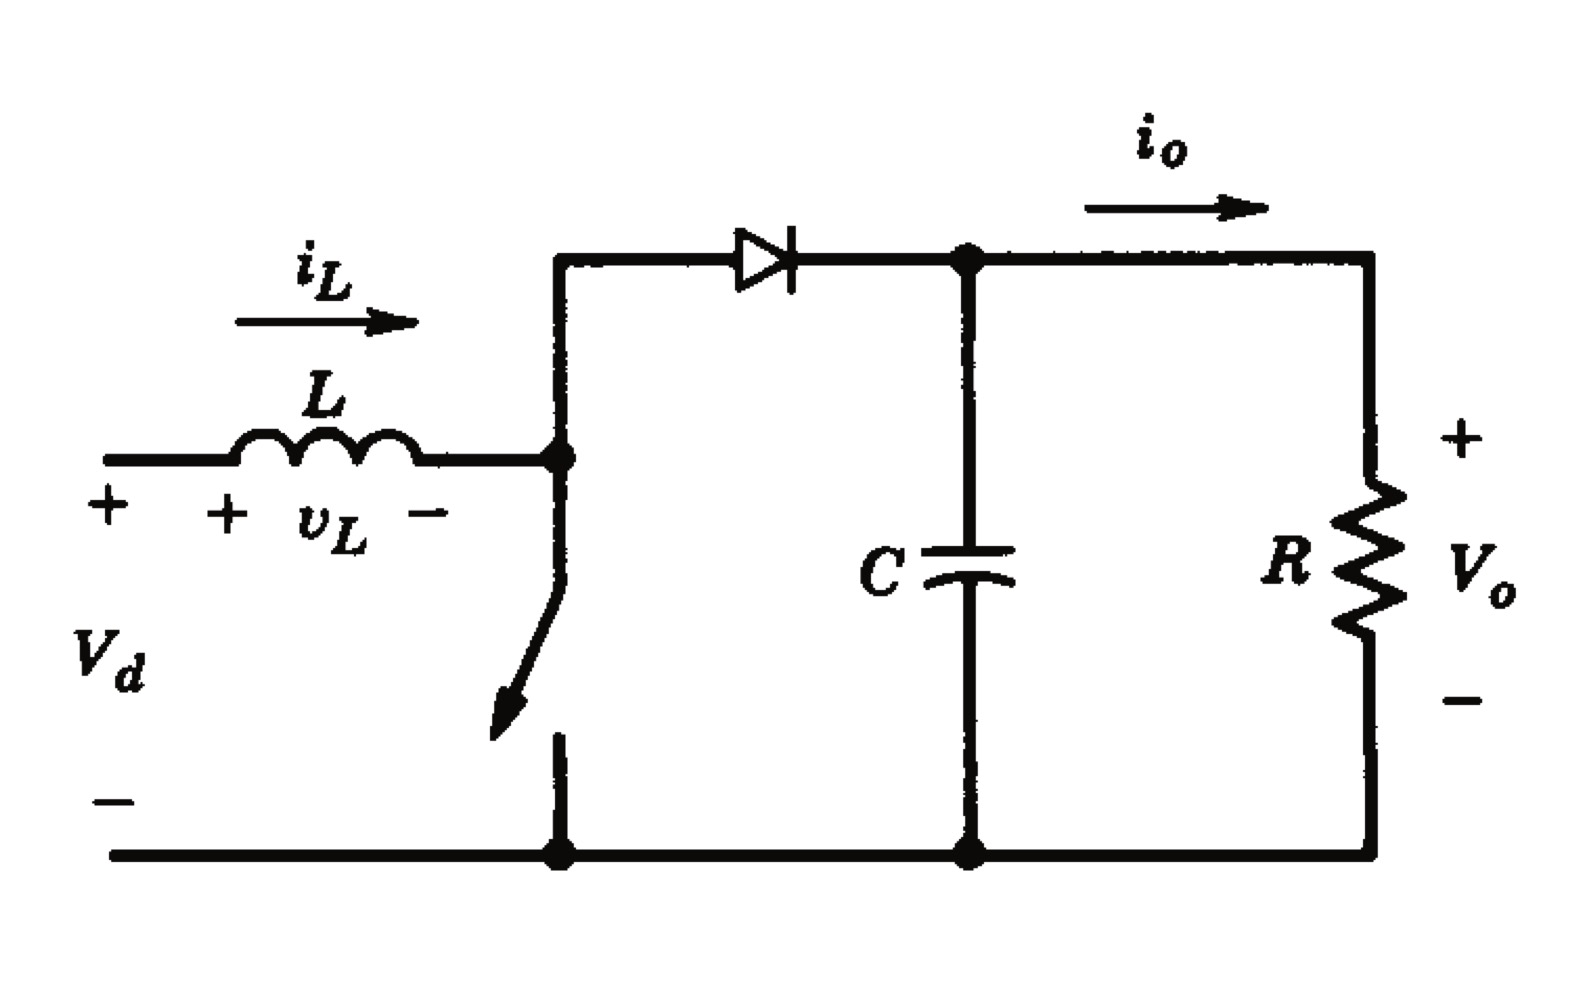
\includegraphics[width=0.5\linewidth]{IMAGES/Indus_el/IMG_0177.jpeg}
\end{figure}

During $t_{on}$, the switch is on and the diode is off. During $t_{off}$ it is the opposite. \\

The \textbf{duty cycle} is defined as : $D = \frac{t_{on}}{T_s}$, with $T_s$ the total period of the switch.\\
During steady-state, the average voltage across the inductor is zero same goes for the capacitor with the current. \\
We then get : $V_d t_{on} + (V_d - V_o)T_{off} = 0$ which gives us the input-output voltage relation of a Boost converter : \begin{equation}
    \frac{V_o}{V_d} = \frac{T_s}{t_{off}} = \frac{1}{1-D} = \frac{I_d}{I_o}
\end{equation}
\warning That last relation is true only if we consider no power losses !

There exists two modes : \begin{itemize}
    \item CCM : (Continuous Conduction Mode) inductor current is flowing continuously\\
    \item DCM : (Discontinuous Conduction Mode) inductor current is zero for a certain period of time\\
\end{itemize}

At the boundary condition, the average inductor current is : $I_{LB} = \frac{T_s V_o}{2L} D(1-D) \rightarrow I_{oB} = \frac{T_s V_o}{2L} D (1-D)^2$\\

\textbf{During DCM,} the $\Delta_1 T_s$ is the time for which the inductor current is reducing to zero and $\Delta_2 T_s$ is the time for which the inductor current/voltage is zero. \\
We have the duty cycle expressed as : \begin{equation}
    D = [\frac{4}{27} \frac{V_o}{V_d} (\frac{V_o}{V_d} -1 ) \frac{I_o}{I_{oB, max}}]^{1/2}
\end{equation}

\textbf{During CCM,} we have $I_L$ the average component equal to the input current and $\Delta I_L$ the peak-to-peak ripple.\\
We have $I_L = I_d = \frac{V_d}{R} \frac{1}{(1-D)^2}$ and therefore, \begin{equation}
L = \frac{V_d}{\Delta I_L} DT_s = \frac{V_o}{\Delta I_L} D(1-D) T_s\end{equation}
\warning It is desired to reduce $\Delta I_L$ in the range of $10\%$ to $20\%$ of $I_L$.\\

For CCM, we assume an average diode current through the load resistor. $\Delta Q$ represents the additional charge and $\Delta V_o$ the peak-to-peak voltage ripple : \begin{equation}\Delta V_o = \frac{\Delta Q}{C} = \frac{V_o}{R} \frac{D T_s}{C}\end{equation}
With $\frac{\Delta V_o}{V_o} = \frac{D T_s}{RC} = \frac{DT_s}{\tau}$\\

Although, we have some parasitic elements. Switches and diodes are not ideal. Inductors have finite resistance of winding $R_L$. \\
\begin{itemize}
    \item $I_{PV}$ PV panel variable current source\\
    \item $C_{PV}$ capacitance at the output of a PV panel\\
    \item $V_{PV}$ PV panel output voltage\\
    \item $I_{C, PV}$ input capacitance current\\
    \item $L_B$ boost converter inductance\\
    \item $V_{L,B}$ instantaneous inductor voltage\\
    \item $R_B$ boost inductor internal resistance\\
    \item $V_{in}$ voltage across the switch\\
    \item $C_{dc}$ output capacitor\\
    \item $V_{dc}$ voltage across the output capacitor\\
    \item $R_{load}$ load at the output is represented as a resistance\\
\end{itemize}
The boost DC-DC converter function is to extract the maximum available power from the PV panels.\\

We can solve the system using Laplace such that : \begin{itemize}
    \item $V_{PV} = \frac{1}{s C_{PV}} I_{C, PV} = \frac{1}{s C_{PV}}(I_{PV} - I_{L,B})$ \warning $I_{PV}$ is controlled by the system and $I_{LB}$ is the one we want to control.\\
    \item Transfer function from the output $V_{PV}$ to the input $I_{L,B}$ : \begin{equation}G_v(s) = \frac{V_{PV}}{I_{PV} - I_{L,B}} = \frac{1}{sC_{PV}}\end{equation}
\end{itemize}

The switching cell can also be analyzed. When the switch S is turned on (defined by D) : $V_{in} = 0$, $V_{L,B} = V_{PV}$.\\
When the switch S is turned off (defined by $1-D$) : $V_{in} = V_{DC} $, $V_{L,B} = V_{PV} - V_{DC}$.\\
Through the duty cycle $1-D$ is $V_{in} = (1-D) V_{DC}$.

Then, the transfer function linking the output $I_{L,B}$ to the input $V_{PV} - V_{in}$ : \begin{equation}
    G_i(s) = \frac{1}{R_B + sL_B} = \frac{I_{L,B}}{V_{PV} - V_{in}}
\end{equation}

\subsubsection{PI controller review}
A first order system is defined by $H(s) = \frac{G}{1+sT}$, with T the time constant that characterizes the rate of change of the output and G the static gain characterizing the final value of the output.\\

We can define \begin{itemize}
    \item $f_B$ the bandwidth as the frequency from which the zero-frequency gain $G(0)$ is attenuated by more than $3dB$
    \item $Q$ the resonance factor as the ratio between the gain corresponding to the maximum of the frequency response curve and the value $G(0)$
    \item the rise time $t_r = \frac{2 to 3}{\omega_B}$
\end{itemize}

A second order system is defined by : $H(s) = \frac{\omega_0^2}{(s-s_1)(s-s_2)}$. Where \begin{itemize}
    \item $\omega_0$ the natural frequency
    \item $\xi$ the damping factor
    \item if $\lvert \xi \rvert <1$m we have complex poles $s= -\xi \omega_0 \pm j \omega_0 \sqrt{1-\xi^2}$, else we have real poles
    \item if $\xi >0$, the system is stable
\end{itemize}

Generally, we have a ratio of two polynomials : $H(s)= \frac{M(s)}{N(s)}$ where for a stable system $n>m$\\
\warning For a system to be asymptotically stable, all the roots of $N(s)$ must be characterized by $\real(s)<0$\\

Let define \begin{itemize}
    \item C(s) controller
    \item A(s), D(s) actuator and/or delay
    \item P(s) plant transfer function
    \item r(s) reference signal
    \item y(s) plant output
    \item e(s) error at the input of a controller
    \item u(s) controller output
    \item d(s) disturbance
\end{itemize}
The open-loop transfer function is : $H_{OL}(s) = C(s) A(s) P(s)$ and the closed loop : $H_{CL}(s) = \frac{H_{OL}(s)}{1+H_{OL}(s)}$\\

The plant transfer function related to the current control is expressed as $P_1(s) = \frac{K_1}{1+sT_1}$ and the TF related to the voltage control $P_2(s) = \frac{1}{sT_2}$.\\

There are numerous delays present in the system (sampling, filters and their delay, computational delay, PWM...).\\
We assume that these delays are smaller than the time constant of the plant $T_1 \simeq (5-10) T_{\sum}$.\\

Therefore, $A(s) = \frac{K_{\sum}}{1+sT_{\sum}} = D(s)$.\\

We use here PI controller that can have the form : $C_{PI}(s) = K_p + K_i \frac{1}{s} = K_p + \frac{1}{sT_i} = \frac{1+sT_n}{sT_i}$\\

\warning For tuning the controllers, we use two criterions Magnitude optimum (MO) and Symmetric optimum (SO).\\

\warning To ensure that the plant output follows the reference, the closed-loop system should have an infinite bandwidth and zero phase shift.\\

\subsubsection{Magnitude optimum}
We want $\lvert H_{CL}(j\omega) \rvert = 1$. \\
We have $H_{OL}(s) = \frac{1+sT_n}{sT_i} \frac{K_{\sum}}{1+sT_{\sum}} \frac{K_1}{1+sT_1}$.\\

We need to cancel the pole at $T_1 \rightarrow T_n = T_1$. Or $H_{OL}(s) = \frac{K_{\sum} K_1}{sT_i( 1+sT_{\sum})}$.\\

Now for $T_i$, we need to look at the denominator of the closed-loop TF and set its absolute value to 1 (neglect high order terms) : $T_i = 2K_{\sum} K_1 T_{\sum}$\\
\begin{equation}
    H_{CL}(s) = \frac{1}{1 + s2 T_{\sum} + s^2 2 T_{\sum}^2}
\end{equation}

\subsubsection{Symmetric optimum}
The symmetrical optimum tuning is applied to plants containing a pure integrator $(\frac{1}{sT_2})$\\

The open-loop TF is : $H_{OL}(s) = \frac{K_{\sum} (1+sT_n)}{s^2 T_i T_2 (1+ sT_{\sum})}$.\\

We only need to apply the $\lvert H(j\omega)\rvert =1$ condition on the closed-loop TF. By neglecting the high order terms, we get $T_n = 4T_{\sum}$ and $T_i = 8 K_{\sum} \frac{T_{\sum}^2}{T_2}$.\\
\begin{equation}
    H_{CL}(s) = \frac{1 + s4 T_{\sum}}{1+s4T_{\sum} + s^2 8 T_{\sum}^2 + s^3 8 T_{\sum}^3}
\end{equation}

\warning The numerator can cause a large overshoot, a reference filter is normally introduced $R_F(s) = \frac{1}{1+sT_n}$.\\

\begin{itemize}
    \item Inner loop should be tuned first either using MO or SO
    \item Outer loop is tuned afterwards using SO
    \item Inner loop is supposed to be fact
    \item Outer loop needs to allow for inner loop to finish its transition and is therefore slower (one order of magnitude)
\end{itemize}

\quad \underline{Inner loop tuned with MO :}\\
$H_{CL}(s) \simeq \frac{1}{1+s2T_{\sum 1}}$ which is a reasonable assumption as $T_{\sum 1}^2$ is very small.\\
The equivalent delay TF $D_{\sum'}(s) = \frac{K_{\sum 2}}{1+sT_{\sum'}}$, $T_{\sum'} = T_{\sum 2} + 2T_{\sum 1}$\\

\quad \underline{Inner loop tuned with SO :}\\
$H_{CL}(s) \simeq 1$ as we ignore high order terms.\\
The equivalent delay TF $D_{\sum'}(s) = \frac{K_{\sum 2}}{1+sT_{\sum'}}$, $T_{\sum'} = T_{\sum 2} + 4T_{\sum 1}$\\

\subsubsection{PI anti-windup}
Actuators have limits, i.e. the DC link voltage of a converter; the maximum peak phase output voltage of a VSI...\\
When designing control system, we need to take the physical limits of our actuators : introduce a limiter or saturation blok at the controller output.\\

Integrator windup phenomenon occurs when the controller output saturates. Even when the controlled variable is the set value, controller still saturates leading to large overshoot.\\

To deal with the presence of actuator saturation we have different approaches : \begin{itemize}
    \item Avoiding saturation of control variable (smoothing of set point changes, detuning the controller)
    \item Conditional integration (limiting the integral term but this cause steady state error, stopping integration term when the error is greater than a threshold, stopping integration when controller saturates)
    \item Back calculation (re-computing integral term when the controller saturates, we use the gain $K_{bc} = \frac{K_i}{K_p}$)
\end{itemize}

\begin{figure}[hbt!]
    \centering
    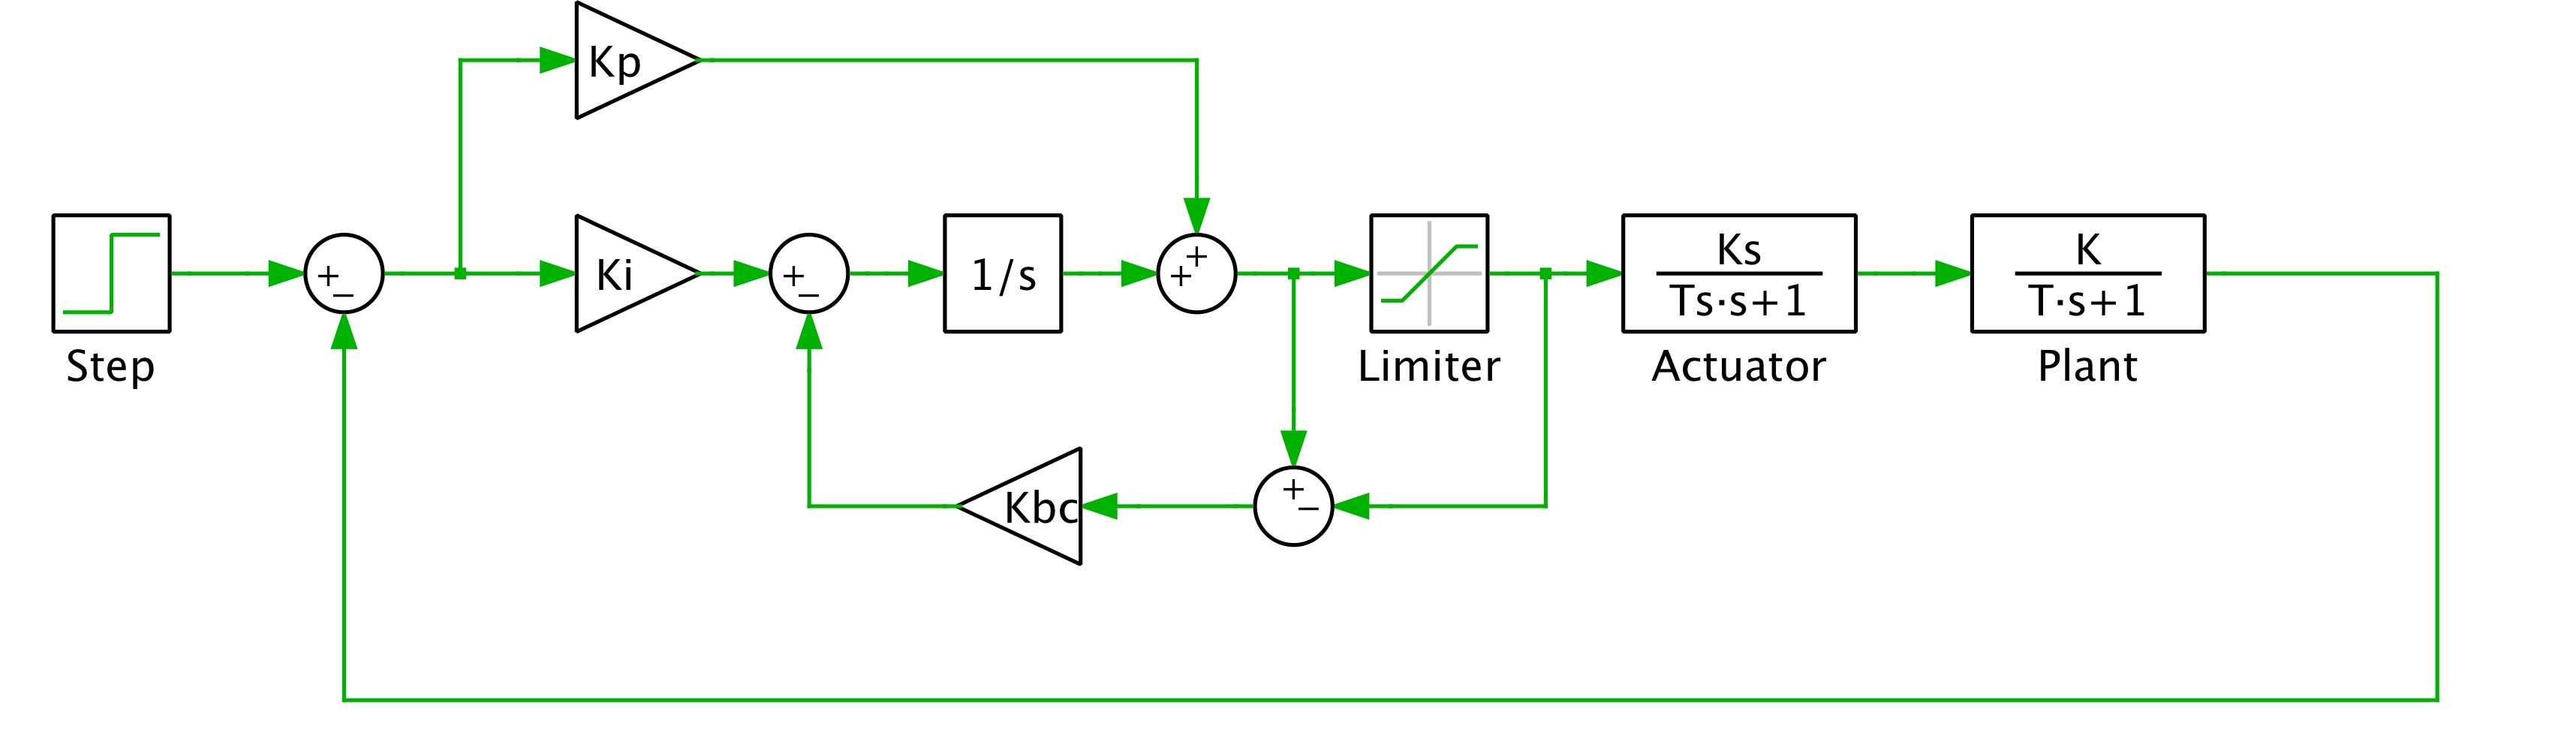
\includegraphics[width=0.7\linewidth]{IMAGES/Indus_el/IMG_0179.jpeg}
    \caption{CL system tuned with MO and regulator Anti-windup}
\end{figure}

\subsubsection{Discretization}
We have the following : \begin{itemize}
    \item ADC - Analog to Digital Converter
    \item ZOH - Zero-Order Hold block maintains controller output constant between samples
    \item Clock - determines the frequency of actions of different block of a system
\end{itemize}

\begin{theorem}
    In order to reconstruct a continuous signal,, the sampling frequency must follow : $f_s > 2f_{max}$.
    In which $f_{max}$ is the maximum frequency to be reconstructed.
\end{theorem}

If this is not respected, it may result in aliasing (or overlapping in the spectrum).\\
\warning The sampling frequency for digital converter system is chosen according to the bandwidth of the CL system \begin{equation}
    f_s \simeq (6 to 25) f_B
\end{equation}

The output of the ZOH is : $h(kT_s + t) = x(T_s)$ and its transfer function is therefore $G_{ZOH} = \frac{H(s)}{X(s)} = \frac{1-e^{-sT_s}}{s}$. (The ZOH can be described as two heavyside unit step : $h(kT_s + t) = H(kT_s) - H(kT_s - T_s)$.\\

The ZOH can be considered as a filter having a frequency response given by : $G_{ZOH}(j\omega) = T_S sinc(\omega T_s/2) e^{-j\omega T_s/2}$. The gain at 0 frequency is $T_s$ but it introduces an attenuation at high frequency ($G_{ZOH}(f_s/2) = 0.637 T_s$)\\

The z-transform is the discrete time equivalent of the laplace transform . \begin{equation}
    \begin{gathered}
        F(z) = \sum_{k=0}^\infty f(kT_s) e^{-k}\\
        z = e^{sT_s}\\
    \end{gathered}
\end{equation}

There are several ways to approximate integral in discrete time system : \begin{itemize}
    \item Explicit Euler Method (forward) $y(kT_s) = y(kT_s - T_s) + x(kT_s - T_s) T_s$
    \item Implicit Euler Method (backward) $y(kT_s) = y(kT_s - T_s) + x(kT_s) T_s$
    \item Trapezoidal Method (tustin) $y(kT_s) = y(kT_s - T_s) + \frac{x(kT_s) + x(kT_s - T_s)}{2} T_s$
\end{itemize}

One property of the Z-transform : $Z(x(t- kT_s)) = z^{-k} X(z)$. 
We have : \begin{itemize}
    \item Forward Euler $s = \frac{1-z^{-1}}{z^{-1} T_s}$
    \item Backward Euler $s = \frac{1-z^{-1}}{T_s}$
    \item Tustin $s = \frac{2}{T_s} \frac{1-z^{-1}}{1+z^{-1}}$
\end{itemize}

\begin{figure}[hbt!]
    \centering
    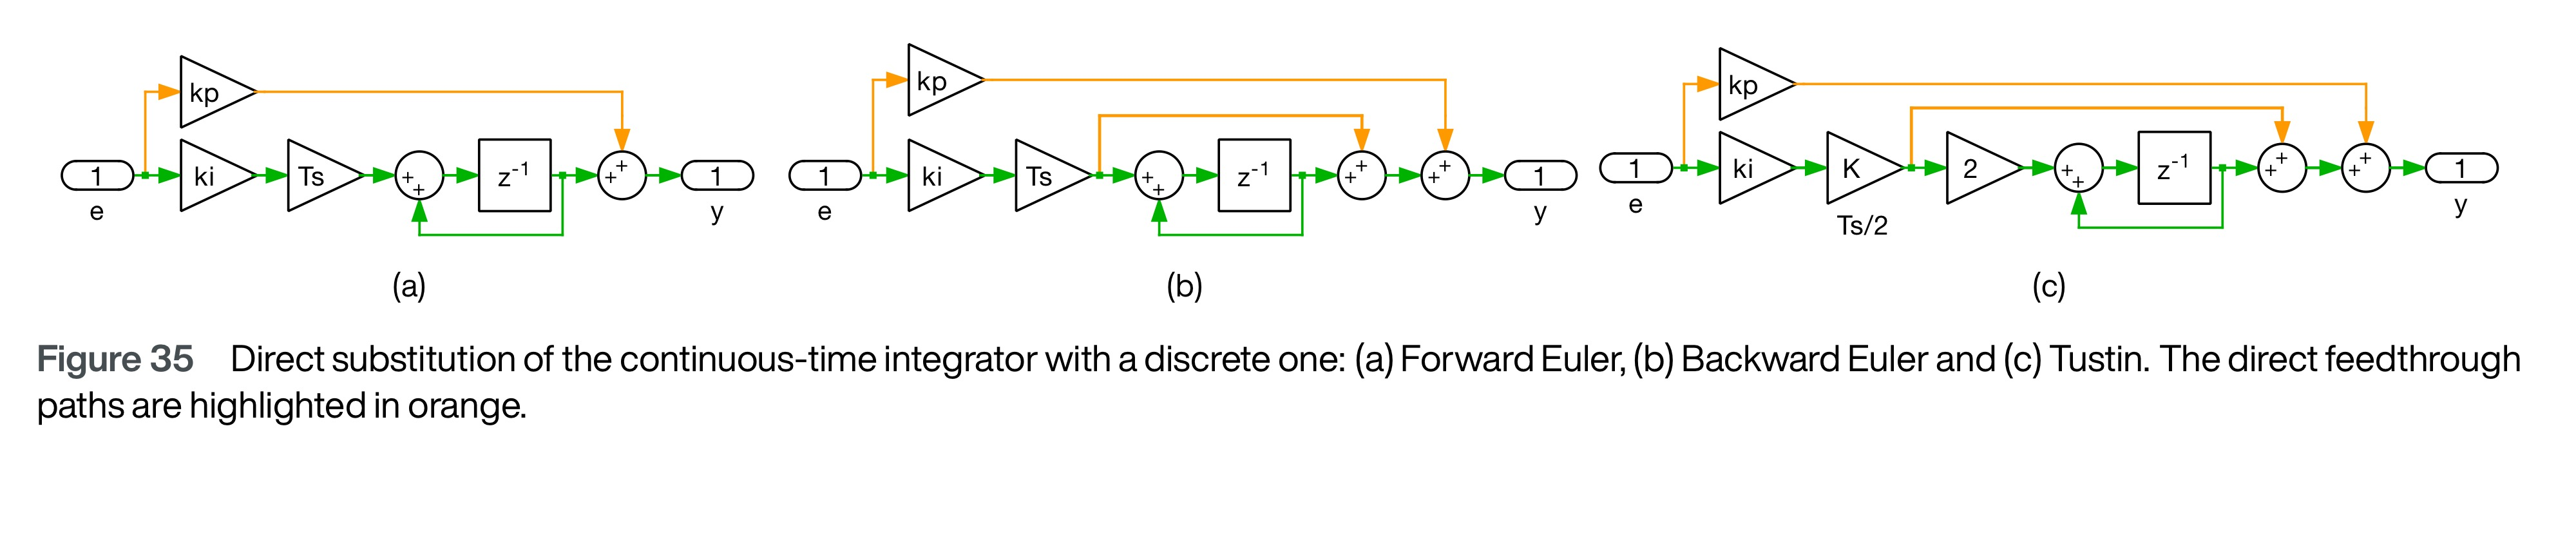
\includegraphics[width=0.9\linewidth]{IMAGES/Indus_el/IMG_0180.jpeg}
\end{figure}

\subsection{Voltage Source Inverter (VSI)}
\subsubsection{AC variable modeling}

To simplify the analysis of three-phase systems we can use \textbf{space vectors} defined as : $v = \frac{2}{3} (v_a + \alpha v_b + \alpha^2 v_c)$ where $v_a$, $v_b$ and $v_c$ are balanced sinusoidal : $v_a + v_b + v_c = 0$. The vector $\alpha$ is defined as $\alpha = e^{j 2\pi/3}$.\\

The system can therefore be represented as : \begin{equation}
    \begin{gathered}
        V_{\alpha \beta 0} = \frac{2}{3} \begin{pmatrix}
            1 & -\frac{1}{2} & -\frac{1}{2}\\
            0 & \frac{\sqrt{3}}{2} & -\frac{\sqrt{3}}{2}\\
            \frac{1}{2} & \frac{1}{2} & \frac{1}{2}
        \end{pmatrix} \begin{pmatrix}
            v_a\\ v_b\\ v_c\\
        \end{pmatrix}\\
        \begin{pmatrix}
            v_\alpha\\ v_\beta\\ 
        \end{pmatrix} = \frac{2}{3} \begin{pmatrix}
            1 & -\frac{1}{2} & -\frac{1}{2}\\
            0 & \frac{\sqrt{3}}{2} & -\frac{\sqrt{3}}{2}\\
        \end{pmatrix} \begin{pmatrix}
            v_a\\ v_b\\ v_c\\
        \end{pmatrix}
    \end{gathered}
\end{equation}

We have the elements : \begin{itemize}
    \item $I_{boost}$ current from the Boost converter
    \item $C_{out}$ DC link capacitor of VSI
    \item $I_s$ current of VSI
    \item $L$ grid filter inductance
    \item $R$ parasitic resistance of a grid filter
    \item $i_a, i_b, i_c$ grid/VSI currents
    \item $v_{ga}, v_{gb}, v_{gc}$ grid voltages
    \item $v_a, v_b, v_c$ VSI voltages
\end{itemize}

\begin{figure}[hbt!]
    \centering
    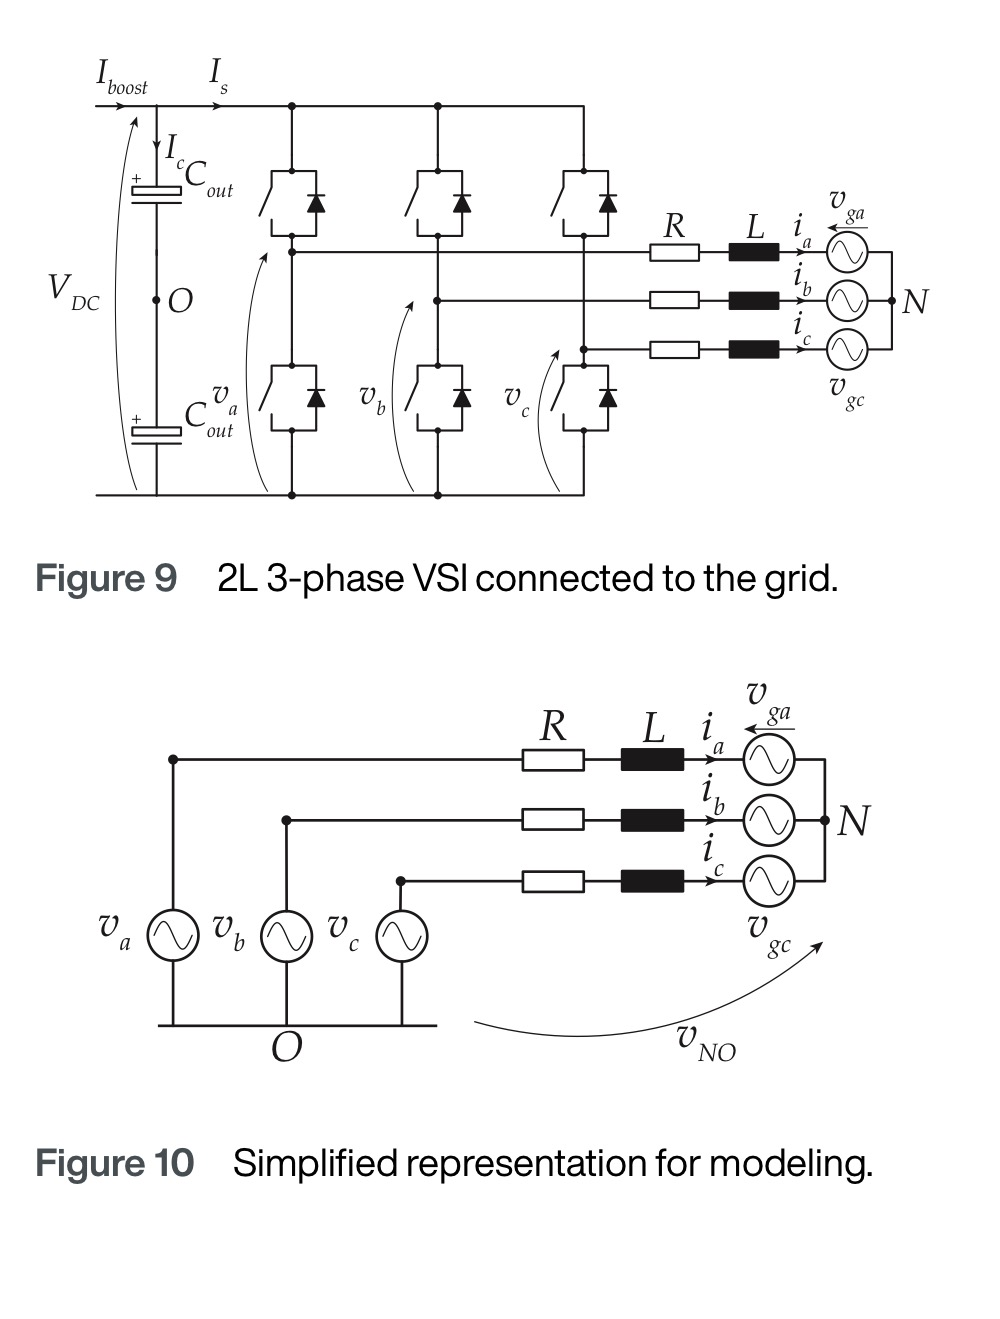
\includegraphics[width=0.7\linewidth]{IMAGES/Indus_el/IMG_0183.jpeg}
\end{figure}

In the $abc$ frame, we have the relations : \begin{equation}
    \begin{gathered}
        si_a = \frac{1}{L}(v_a - v_{ga} - Ri_a)\\
        si_b = \frac{1}{L}(v_b - v_{gb} - Ri_b)\\
        si_c = \frac{1}{L}(v_c - v_{gc} - Ri_c)\\
    \end{gathered}
\end{equation}

Because the neutral isn't connected between the grid and VSI, we can use \textbf{Clarke Transform} ($v_\alpha, v_\beta$) to represent AC variables a space vectors.

This simplifies the system to one equation : $\underline{v}_{\alpha\beta} = R \underline{i}_{\alpha\beta} + L\frac{d \underline{i}_{\alpha \beta}}{dt}+ \underline{v}_{g\alpha \beta}$.\\

But this reference frame isn't optimal as we have to deal with AC variables. We then choose a rotating reference frame $dq$ that rotates with the grid.\\

\begin{equation}
    \begin{gathered}
        \underline{v}_{dq} = \underline{v}_{\alpha\beta} e^{-j\theta_k}\\
        \begin{pmatrix}
            v_d\\ v_q\\
        \end{pmatrix}= \begin{pmatrix}
            \cos \theta_k & \sin \theta_k\\
            -\sin \theta_k & \cos \theta_k\\
        \end{pmatrix} \begin{pmatrix}
            v_\alpha \\ v_\beta\\
        \end{pmatrix}\\
        \theta_k = \omega t + \theta_0
    \end{gathered}
\end{equation}

This enables us to have the system equation in DC form : \begin{equation}
    \underline{v}_{dq} = R \underline{i}_{dq} + L \frac{d\underline{i}_{dq}}{dt} + j\omega L \underline{i}_{dq} + \underline{v}_{gdq}
\end{equation}

With (assuming initial conditions $\theta_0 = 0$) : $\underline{v}_{\alpha \beta} = \underline{v}_{dq} e^{j\omega t}$, $\underline{i}_{\alpha \beta} = \underline{i}_{dq} e^{j\omega t}$, $\underline{v}_{g\alpha \beta} = \underline{v}_{gdq} e^{j\omega t}$.\\

The plant model for grid current control is similar to that of Boost ($T = \frac{L}{R}$, $K = \frac{1}{R}$) : $G_i(s) = \frac{K}{1+sT}$.\\

We also have : $G_v(s) = \frac{V_{DC}}{I_{boost} - I_s} = \frac{1}{sC_{out}}$.\\

We also need to take into account a small order delay with a gain : $G_{pe} (s) = \frac{K_{pe}}{1+sT_{pe}}$.

\subsubsection{PWM}
We can either have symmetrical sampling : reference is sampled at the beginning of the PWM period, the resulting pulse is centered around the middle and the time delay associated with the sampling is $T_s/2 = T_{sw}/2$.

Or asymmetrical : reference is sampled at the beginning and middle of the PWM period, the pulse is not centered around the middle and the time delay is $T_s/2 = T_{sw}/4$.\\

To prevent short circuit we need to take into account : \begin{itemize}
    \item semiconductors have finite switching times
    \item two switch cannot conduct simultaneously 
    \item dead-time duration depends on semiconductors technology (MOSFET : 100ns, IGBT : 1 $\mu$s)
\end{itemize}

\begin{figure}[hbt!]
    \centering
    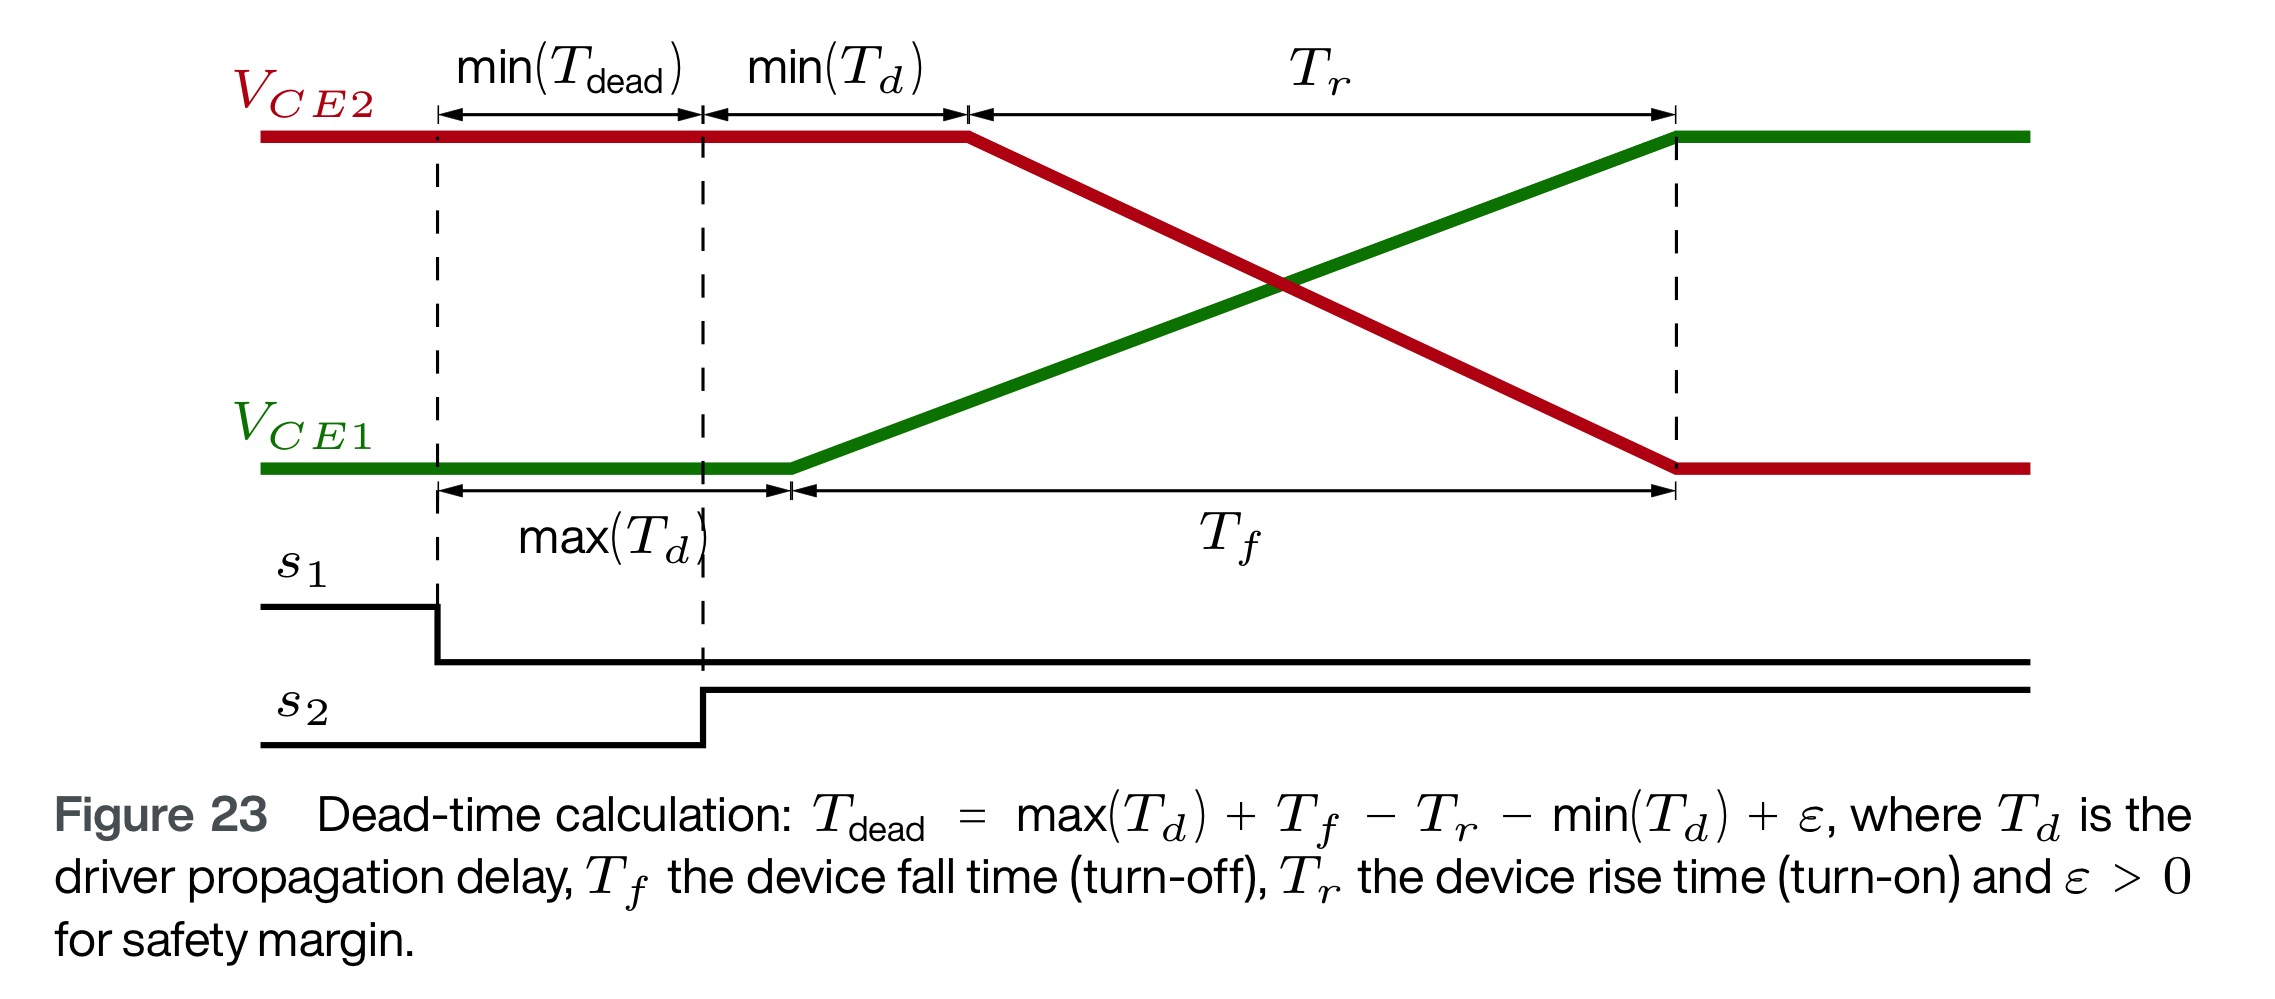
\includegraphics[width=0.7\linewidth]{IMAGES/Indus_el/IMG_0184.jpeg}
\end{figure}
\subsubsection{3-phase VSI}

\begin{figure}[hbt!]
    \centering
    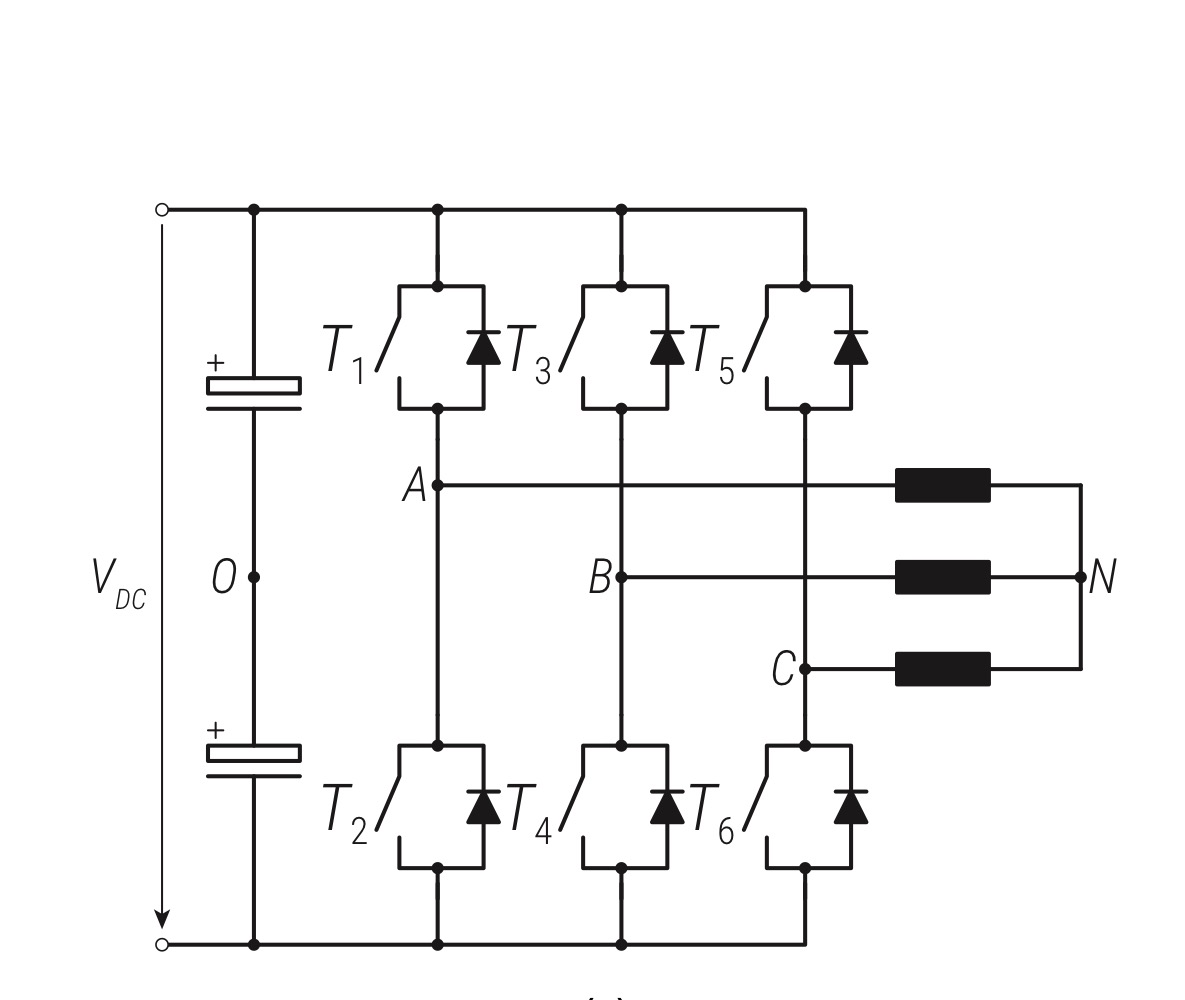
\includegraphics[width=0.7\linewidth]{IMAGES/Indus_el/IMG_0187.jpeg}
\end{figure}

This is the representation of a double stage three-phase inverter. It has 8 switch combinations and all the components need to add up to zero.\\

The \textbf{modulation index} is defined as $M = \frac{V_m}{V_{DC}/2}$. The fundamental three-phase reference signals are $v_i^* = V_m \cos(\omega t + \varphi)$ with $i = \{a,b,c\}$. The normalized version is then : $m_a^* = M\cos(\omega t + \varphi)$.\\

The goal is to compare a reference signal with a carrier signal to trigger the different switches. 

Normally, we have carrier bounded to $\pm 1$ range. \\
Sinusoidal PWM (SPWM) is bounded by $M_{max} = 1$ otherwise low-order harmonics appear.\\

\subsubsection{Overmodulation}

As M becomes larger than 1, we have some \textbf{overmodulation} and the switches cannot switch anymore as the system is saturated. Harmonics then appear and deform the output current.\\

Each leg is driven by $180^\circ$ pulse. The voltage with respect to the negative terminal is then $v_A(t) = V_{DC} \frac{2}{\pi}(\frac{\pi}{4} + \frac{1}{3} \sin(3\omega_0 t) + \frac{1}{5} \sin(5\omega t) + \cdots )$. The magnitudes of the harmonics are $V_{DC} \frac{2}{\pi} \frac{1}{k}$.\\
The line-to-line voltage are then $v_{ab}(t) = V_{DC} \frac{2\sqrt{3}}{\pi} (\sin(\omega_0 t + \pi/6) + \frac{1}{5} \sin (\omega_0 t - \pi/6 + \cdots)$ and the magnitudes of the harmonics are $V_{DC} \frac{2\sqrt{3}}{\pi} \frac{1}{k}$.\\

One positive aspect of overmodulation of the gain in fundamentals despite the appearance of harmonics. One general limit is $M = 1.27$.\\

\subsubsection{Zero-sequence injection}
Adding something equal to all three phases does not change anything on the output as they compensate. We can then allow $M_{max}>1$ without the appearance of harmonics.\\

For example, we can do a third harmonic injection as it is the most likely to have a large impact : $m_a^* = M\cos(\omega t) + bM \cos(3\omega t)$. To find b set the derivative to 0 and $b= -\frac{1}{6}$ (maximum at $\omega = \frac{\pi}{6}$). We then have $M_{max} = 1.15$\\

One other injection type is the min/max signal injection. It is not always convenient to inject a third harmonic so instead we add a min/max signal.


\subsubsection{DPWM}
Discontinuous PWM (DPWM) acts on the switches depending on the load type. It avoids switching for a certain time in a period. We get here $M_{max} = 2/\sqrt{3}$.\\

There exists multiple ways : DPWMMIN, DPWMMAX, DPWM0, DPWM1, DPWM2, DPWM3 each with a different way of switching (most are the symmetry of another one).\\

The presence of harmonics also greatly depends on the switching frequency.

\begin{figure}[hbt!]
    \centering
    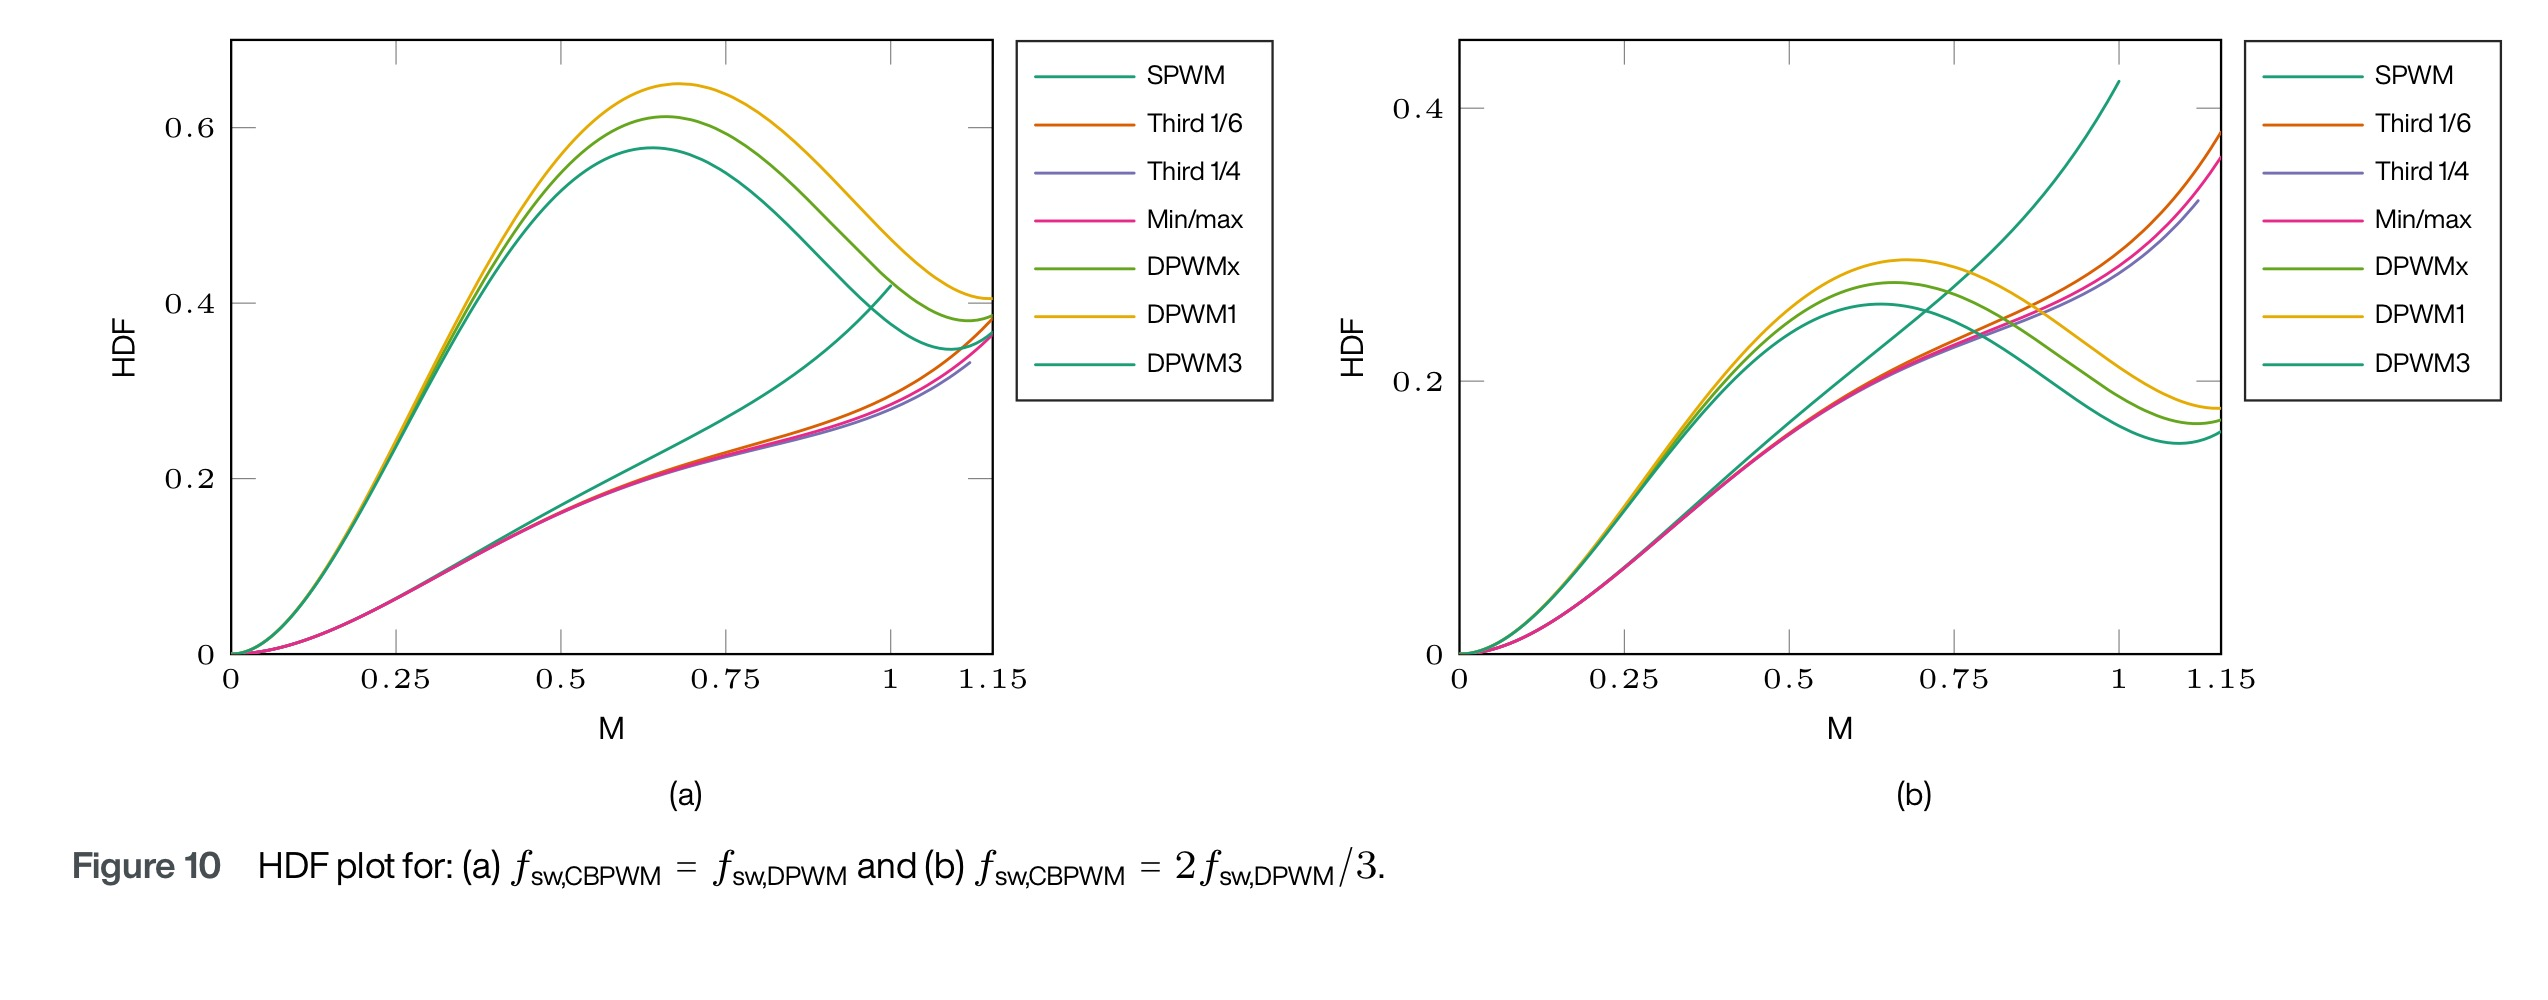
\includegraphics[width=0.8\linewidth]{IMAGES/Indus_el/IMG_0188.jpeg}
\end{figure}

In overmodulation region, the real modulation index is not anymore a linear expression from the desired modulation index.\\

\subsubsection{Multilevel converters}
We can also have multilevel converters which offer higher DC link voltage with lower switching frequency but have a higher complexity in the modulator.\\
In practice, we never go above 5 levels.

\subsubsection{Space vector PWM}
For the converter, we can either use a carrier based PWM that uses an external carrier signal to modulate the output or we can use space vector PWM method that acts on the $\alpha-\beta$ plane.\\

A 2level-3phase inverter has 8 different possible output for the phases. They can all be described in the $\alpha-\beta$ plane with $V = \frac{2}{3} (V_A + \alpha V_B + \alpha^2 V_C)$ with $\alpha = e^{j\frac{2\pi}{3}}$.\\
There are two zero vectors $V_0, V_7$ and six active space vectors $V_1, V_2, V_3, V_4, V_5, V_6$.\\

They form an hexagon and split the $\alpha \beta$ plane into six sectors, each spanning $60^\circ$.\\
We can also define the reference space vector as $v_{\alpha \beta}^* = M \frac{V_{DC}}{2}e^{j\theta}$, $\theta = \omega t$. It represents the desired inverter output voltage.\\

\begin{figure}[hbt!]
    \centering
    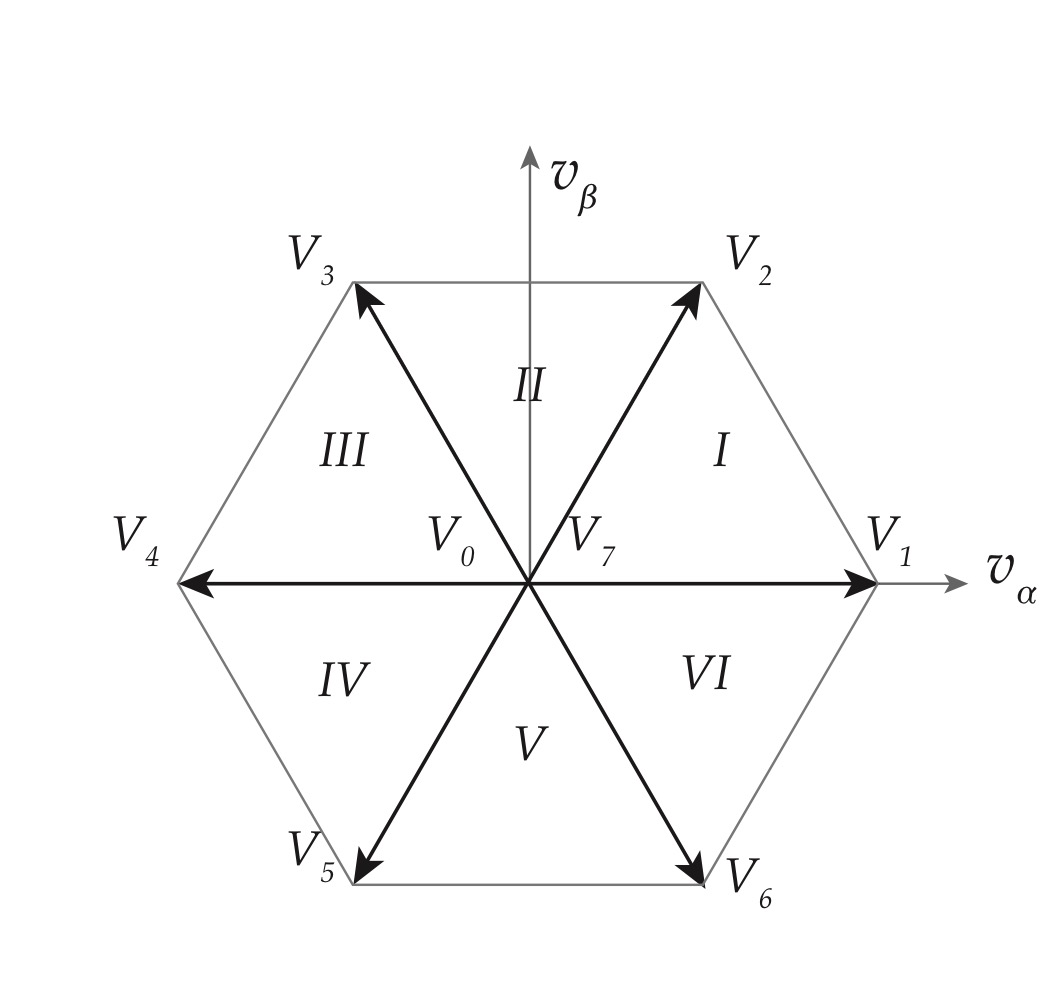
\includegraphics[width=0.6\linewidth]{IMAGES/Indus_el/IMG_0189.jpeg}
    \caption{Space vectors and sectors in $\alpha\beta$ plane}
\end{figure}

To simplify, we can normalize the active space vectors with $\frac{V_{DC}}{2}$ : \begin{itemize}
    \item $V_1 = \frac{4}{3}$
    \item $V_2 = \frac{4}{3} e^{j\pi/3}$
    \item $V_3 = \frac{4}{3} e^{j 2\pi/3}$
    \item $V_4 = \frac{4}{3} e^{j \pi}$
    \item $V_5 = \frac{4}{3} e^{j 4\pi/3}$
    \item $V_6 = \frac{4}{3} e^{j5 \pi/3}$
    \item $v_{\alpha \beta}^* = Me^{j\theta}$
\end{itemize}

The goal is to describe the reference space vectors with two adjacent active space vectors : $v_{\alpha \beta}^* T_s = V_1 T_1 + V_2 T_2$.\\
We have in the case of the first sector : $\begin{matrix}
    T_1 = M \frac{\sqrt{3}}{2} \sin(\pi/3 - \theta) T_s\\
    T_2 = M \frac{\sqrt{3}}{2} \sin (\theta) T_s
\end{matrix}$

The remaining time is allocated to zero-space vectors (divided equally) : $T_s - T_1 - T_2 = 2T_0 = 2T_7 = T_{ZSV}$. \\
We then get the duty cycles by normalizing them by the switching time $T_s$ : $\begin{matrix}
    \delta_1 = M \frac{\sqrt{3}}{2} \sin(\frac{\pi}{3}- \theta)\\
    \delta_2 = M \frac{\sqrt{3}}{2} \sin \theta\\
    \delta_0 = \delta_7 = \frac{1}{2} - M \frac{\sqrt{3}}{4} \cos(\frac{\pi}{6} - \theta)\\
\end{matrix}$

\quad \underline{In which order should we apply the space vectors?}\\
Normally, we try to do symmetrical switching sequence to minimize the number of commutations. Sequence start and end with $V_0$ and $V_7$ should be placed at the center.\\

\begin{itemize}
    \item Odd sectors : starting with $V_x$, ending with $V_y$ : \begin{equation}
        V_0 - V_x - V_y - V_7 - V_y - V_x - V_0
    \end{equation}
    \item Even sectors : \begin{equation}
        V_0 - V_y - V_x - V_7 - V_x - V_y - V_0
    \end{equation}
\end{itemize}


DC bus utilization : \begin{itemize}
    \item Increasing M brings tip of the reference space vector closer to the hexagon
    \item linear modulation region is defined by inscribed circle inside the hexagon
    \item overmodulation : tip outside of the hexagon
    \item at limit reference vector will touch hexagon at $\theta = \frac{\pi}{6}$ $(\delta_0 = 0)$
\end{itemize}


Let's define the sector s. We then have $\begin{matrix}
\delta_1 = M \frac{\sqrt{3}}{2} \sin( s \frac{\pi}{3} - \theta)\\
\delta_2 = M \frac{\sqrt{3}}{2} \sin(\theta- (s-1) \frac{\pi}{3})\\
\delta_0 = \delta_7 = \frac{1}{2} - M \frac{\sqrt{3}}{4} \sin((2s-1) \frac{\pi}{6} - \theta)\\
\end{matrix}$

\warning Triangular (min-max) zero sequence signal is equivalent to SVPWM.\\

\quad \underline{Implementation :}\\
\begin{enumerate}
    \item Determine the sector
    \item Compute duty cycle for active space vectors
    \item Compute duty cycle for zero space vectors
    \item Assemble switching pattern
    \item send the PWM signal out
\end{enumerate}


We have for example in sector $s= 1$ (similar in odd sectors) : \begin{itemize}
    \item leg signal $m_A$ has a duty cycle $\delta_A = \delta_7 + \delta_2 + \delta_1$
    \item leg signal $m_B$ has a duty cycle $\delta_B = \delta_7 + \delta_2$
    \item leg signal $m_C$ has a duty cycle $\delta_C = \delta_7$
\end{itemize}

For sector $s=2$ (similar in even sectors): \begin{itemize}
    \item leg signal $m_A$ has a duty cycle $\delta_A = \delta_7 + \delta_2$
    \item leg signal $m_B$ has a duty cycle $\delta_B = \delta_7 + \delta_2 + \delta_3$
    \item leg signal $m_C$ has a duty cycle $\delta_C = \delta_7$
\end{itemize}

\subsubsection{PI regulators}
PI controller do not generally work well with AC signals. They output a phase lag as well as a gain difference.\\

A solution is to use a regulator with hysterisis : the controller does not act when the signal is between two references. It is good for following a reference but the ripple is not constant as the frequency is not constant.\\

Assume the plant model is known : $P_1(s) = \frac{i(s)}{v_0(s) - v_g(s)} = \frac{K_1}{1+sT_1}$, $K_1 = \frac{1}{R}$, $T_1 = \frac{L}{R}$. The converter is represented by a gain : $A_1(s) = 1 = K_{\sum}$.\\

The closed loop TF is therefore : $i(s) = i^*(s) \frac{C(s) A_1(s) P_1(s)}{1+ C(s) A_1(s) P_1(s)} - v_g(s) \frac{P_1(s)}{1+C(s) A_1(s) P_1(s)}$\\

We then have two distinct terms : \begin{itemize}
    \item Reference tracking, we want $\frac{i}{i^*} \simeq 1$ (first term of the TF)
    \item Disturbance rejection, we want $\frac{i}{v_g} \leq \varepsilon$
\end{itemize}
One solution is to make $C(s)$ as large as possible.\\

\quad \underline{Maximum PI gains in stationary $\alpha \beta$ frame :}\\
The open-loop TF is : $H_{OL}(s) = \frac{K_p K_1 K_{\sum}}{\tau_i} \frac{1}{s} e^{-sT_d} \frac{1+sT_i}{1+sT_1}$ with $e^{-sT_d}$ the delay of the converter.\\
Because we want this to be unity at a specific frequency, we get \begin{equation}
    \begin{gathered}
        K_p = \frac{\omega_{c(max)} T_1}{K_1 K_{\sum}}\\
        T_i = \frac{\tau_i}{K_p} \simeq \frac{10 K_{\sum}}{\omega_{c(max)}^2 L}
    \end{gathered}
\end{equation}

The delay caused by a PWM can either be $T_d = 1.5 T_s$ for a single update PWM or $T_d = 0.75 T_s$ for a double update one.\\

\warning The grid voltage is predictable and its effect can be reduced by feedforwarding it. The closed loop TF then becomes : $i(s) = i^*(s) \frac{C(s) A_1(s) P_1(s)}{1+ C(s) A_1(s) P_1(s)} - v_g(s) \frac{(1-F(s) A_2(s))P_1(s)}{1+C(s) A_1(s) P_1(s)}$. With a perfect estimation ($F(s) = 1$), the influence of the grid voltage can be eliminated.

\subsubsection{PR regulators}
The limitation of a PI controller is high at the fundamental reference frequency $\omega_0$. One solution is to increase the controller gain at this frequency. This is possible with a Proportional Resonant (PR) controller : \begin{equation}
    C_{PR}(s) = K_p + K_i \frac{s}{s^2 + \omega_0^2}
\end{equation}

We have that for low and high frequency behaviors approximate a Proportional controller $C_P$. Near infinite gain at the target AC frequency and near zero tracking error and disturbance error at this frequency. However, they can be sensitive to mismatch between the resonant term and the AC fundamental frequency. We therefore use the non-ideal form : \begin{equation}
    C_{PR} (s) = K_p + K_{ni} \frac{2 \omega_b s}{s^2 + 2\omega_b s + \omega_0^2}
\end{equation}
Where $\omega_b$ is the bandwidth around $\omega_0$, $K_{ni} = \frac{K_i}{2\omega_b}$.\\

\begin{itemize}
    \item An ideal PR regulator has a high and sharp resonant peak with very high gain at $\omega_0$
    \item A non-ideal PR regulator has a dampened and widened resonant peak.
\end{itemize}
As a PR only works for one specific frequency, multiple ones are usually set in parallel.\\

\quad \underline{Discretization :}\\
For a perfect discretization, we should apply a forward Euler for the inner integrator and a backward Euler for the outer integrator. 

\subsection{Phase Locked Loop (PLL)}

\subsubsection{Grid synchronization}
Different techniques :\begin{itemize}
    \item Frequency-domain detection methods : based on Fourier Transform (Fourier series, discrete FT, recursive discrete FT)
    \item Time-domain detection methods : based on some adaptive loop to track components on interest (PLL, FLL)
\end{itemize}

\quad \underline{Fourier series (usually not implemented):}\\

Multiplication of unknown sine/cosine signal by an unitary sine/cosine signal gives a DC part if the frequencies are the same and an AC part at double the frequency if the frequencies are the same.\\

Then, we can develop an adaptive filter. The amplitude and phase-angle at frequency of interest are : $V_n' = \begin{cases}
    V_n = \sqrt{a_n^2 + b_n^2}\\
    \theta_n = \arctan \frac{b_n}{a_n}
\end{cases}$

The mean value of the signal is obtained using a low pass filter. The lowest frequency of interest is the grid frequency. At LPF input, the lowest frequency is the double. The LPF cut-off frequency should be one order of magnitude lower. The filter is of the form : $\frac{\omega}{\omega+s}$.\\
\warning Very slow dynamic response of the system.\\
The complex form of the Fourier series can also be used. \\

The DFT is defined as : $V(n) = \sum_{k=0}^{N-1} v(k) e^{-j2\pi \frac{k}{N}n}$.\\
The DFT could be used to extract fundamental frequency component of the grid voltage, however it is computationally demanding.\\

\quad \underline{Phase Locked Loop :}\\

It is a closed-loop system in which an internal oscillator is controlled to keep the time of some external periodic signal through the feedback loop. Consists of : \begin{itemize}
    \item Phase detector (PD) : the output signal is proportional to the phase difference between input signal $v$ and signal generated by an internal oscillator $v'$
    \item Loop Filter (LF) : it has a low pass filter, first order LPF or PI controller
    \item Voltage controller oscillator (VCO) : generates at its output an AC signal whose frequency is shifted wrt a given central frequency $\omega_c$.
\end{itemize}

The PDF as a simple multiplier, LF as a PI controller, VCO as a sinusoidal function : \begin{itemize}
    \item input signal : $v(t) = V\sin(\omega t + \Phi)$
    \item VCO signal : $v'(s) = \cos(\omega' t + \Phi')$
    \item PD output : $\varepsilon_{pd} = V k_{pd} \sin(\omega t + \Phi) \cos( \omega' t + \Phi')$
\end{itemize}

The LF cancels high-frequency terms and assuming VCO is well-tuned $\omega \simeq \omega'$ and $\Phi \simeq \Phi'$ we have : $\overline{\varepsilon}_{pd} = \frac{Vk_{pd}}{2} (\theta - \theta')$, $\theta = \omega t + \Phi$.\\

\begin{figure}[hbt!]
    \centering
    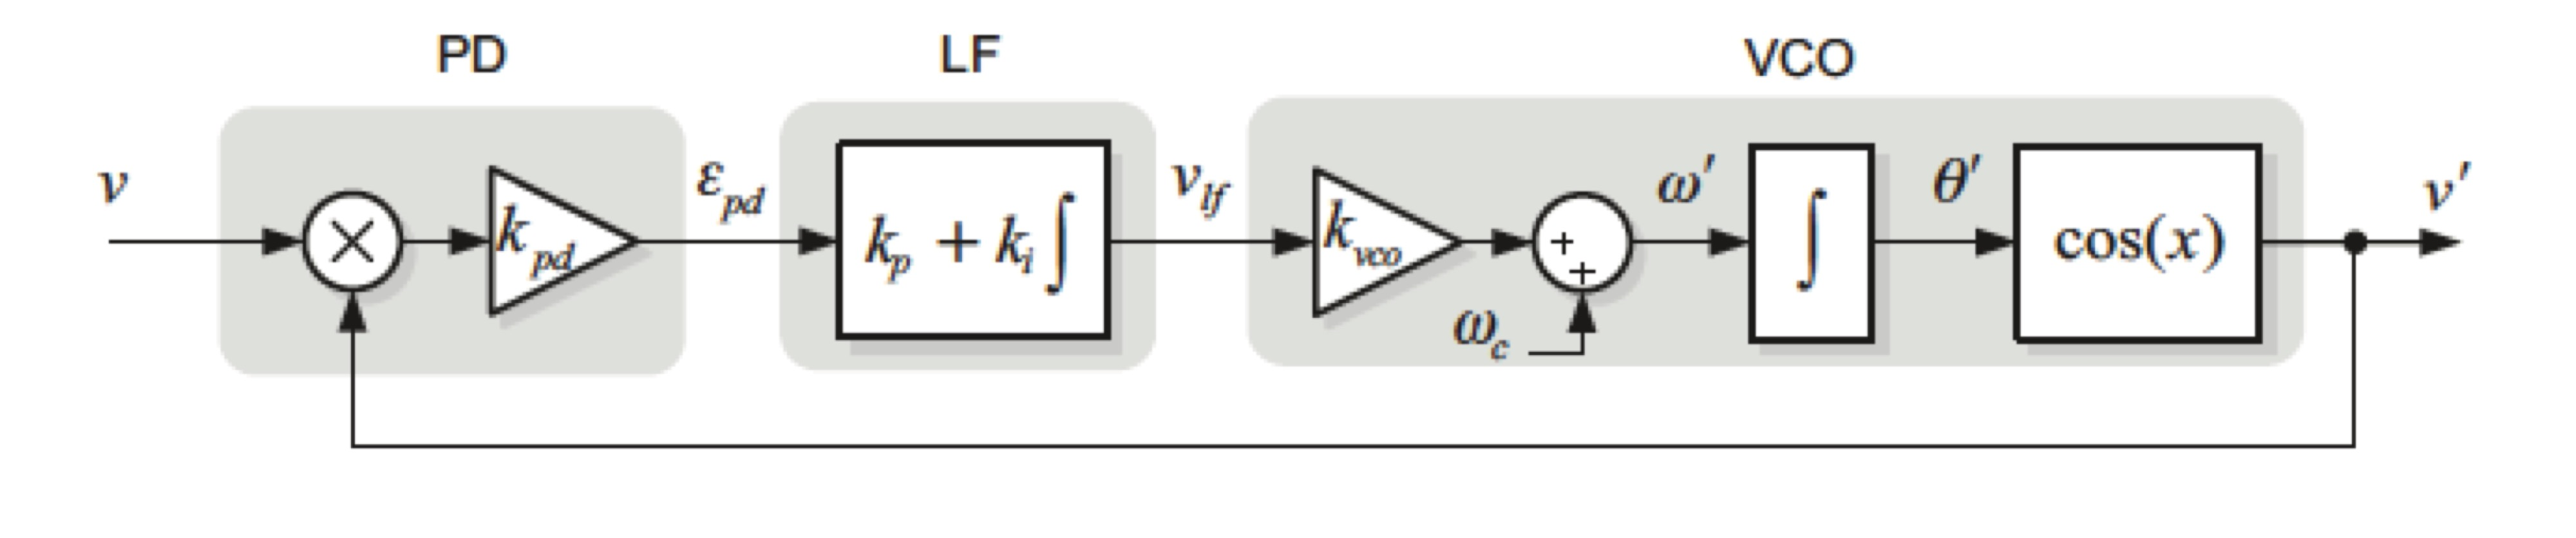
\includegraphics[width=0.7\linewidth]{IMAGES/Indus_el/IMG_0192.jpeg}
    \caption{Block diagram of an elementary PLL}
    \label{fig:elemPLL}
\end{figure}

The average frequency of the VCO is determined as : $\overline{\omega}' = \omega_c + \Delta \omega' = \omega_c + k_{cvco} \overline{ v}_{lf}$. ($\omega_c$ the center frequency, normally the grid frequency).\\

This can be linearized with the following functions : \begin{itemize}
    \item PD : $E_{pd}(s) = \frac{V k_{pd}}{2} (\Theta(s) - \Theta'(s))$
    \item LF : $V_{lf}(s) = k_p (1 + \frac{1}{T_is}) E_{pd}(s)$
    \item VCO : $\Theta'(s) = \frac{1}{s}K_{vco} V_{lf}(s)$
\end{itemize}

By considering $k_{pd} = 2$, $k_{vco} = 1$ and $V=1$, the OL TF is given by : \begin{equation}
    H_{OL}(s) = PD(s) LF(s) VCO(s) = k_p (1+ \frac{1}{T_is}) \frac{1}{s}
\end{equation}

The corresponding CL TF is then : \begin{equation}
    H_{CL}(s) = \frac{k_p s + \frac{k_p}{T_i}}{s^2 + k_p s + \frac{k_p}{T_i}}
\end{equation}

As the $H_{OL}$ has two poles at origin, it is able to track a constant slope ramp without any steady state error. $H_{CL}$ has a LPF.\\

The closed loop TF of $E_{pd}$ is also given by : $E_{CL}(s) = 1- H_{CL}(s) = \frac{s^2}{s^2 + k_ps + \frac{k_p}{T_i}}$.\\

We have : $\omega_n = \sqrt{\frac{k_p}{T_i}}$ and $\xi = \frac{\sqrt{k_pT_i}}{2}$. \begin{itemize}
    \item settling time : $t_s = 4.6 \tau$ (for $\pm 1\% FV$) with $\tau = \frac{1}{\xi \omega_n}$
    \item PI regulator : $k_p = 2\xi \omega_n = \frac{9.2}{t_s}$, $T_i = \frac{2\xi}{\omega_n} = t_s \frac{\xi^2}{2.3}$
\end{itemize}

\quad \underline{PLL response :}\\
If $\omega_c$ is set to 0, then the settling time tends to be really large and we get around $10\%$ error in the output frequency (oscillating frequency because of a second harmonic).\\
By setting $\omega_c$ to the grid frequency (i.e. $50$Hz), the settling time is around what we computed.\\
Several parameters are used to describe PLL performance : \begin{itemize}
    \item Hold range : $\Delta \omega_H= k_{pd} k_{vco} LF(0)$ (frequency at which PLL is able to keep itself phase locked)
    \item Pull-in range $\Delta \omega_P $ (frequency range at which the PLL will always became locked) : $T_P = \frac{\pi^2}{16} \frac{\Delta w_{in}^2}{\xi \omega_n^3}$, $\Delta \omega_{in}$ the variation in input frequency
    \item Lock range $\Delta \omega_L = 2\xi \omega_n$ (frequency range within which PLL locks within one single-beat not between the reference frequency and the output frequency)
    \item Pull-out range $\Delta \omega_{PO} = 1.8 \omega_n (\xi + 1)$ (dynamic limit for stable PLL)
\end{itemize}

\warning A simple multiplier PD is not sufficient to cancel out signal at twice the grid frequency.\\

\quad \underline{PLL based on quadrature signal generator :}\\
Assume the input signal : $v(t) = V \sin(\theta)$. \\
The in-quadrature signal using Quadrature Signal Generator (QSG) is then : $v_{iq}(t) = -V \cos(\theta)$.\\
Then, the PD based on QSG would cancel-out the oscillations at twice the input frequency : $\varepsilon_{pd} = V\sin(\theta) \cos(\theta') - V \cos(\theta) \sin(\theta') = V\sin( \theta - \theta')$.\\

\warning We can use the Park Transform in $\theta'$ to compute it. For instance, $\begin{pmatrix}
    v_d\\ v_q 
\end{pmatrix} = \begin{pmatrix}
    \cos \theta' & \sin \theta'\\
    - \sin \theta' & \cos \theta'
\end{pmatrix}  \begin{pmatrix}
    v_{\alpha}\\ v_{\beta}
\end{pmatrix} = V \begin{pmatrix}
    \sin ( \theta - \theta')\\
    -\cos( \theta - \theta')
\end{pmatrix}$
Where $v_{\alpha \beta} = V \begin{pmatrix}
    \sin \theta\\ -\cos \theta
\end{pmatrix}$
Then, we can either choose to align with the q-axis or the d-axis. Once PLL is locked, grid voltage is real variable in dq frame. We will work with LF in q-axis such that $i_d$ control active and $i_q$ reactive power.

Other ways to implement QSG : \begin{itemize}
    \item PLL based on $T/4$ transport delay : T being the grid fundqmental period (simplest QSG). if grid frequency changes, fixed transport delay will result in error.
    \item PLL based on Hilbert transform : shift $\pm 90^\circ $ phase-angle of input signal depending on its sign. Only affects the phase and not the amplitude
    \item PLL based on the Inverse Park Transform : in-quadrature image of the input signal can be achieved. Filter is introduced in the loop of direct and inverse park transform.
\end{itemize}

\quad \underline{PLL in 3-phase systems :}\\
To generate the QSG, one can use the Clarke Transform to obtain an $\alpha\beta$ signal. Then the Park transform can be used as before for PD.

In addition to basic PPL based on in-quadrature signal, there are implementations based on adaptive filtering. The grid isn't always balanced.\\

\subsubsection{Adaptive noise cancelling}
Inherent second harmonic component in PLL output can be filtered by a QSG.\\
Let $v = s+n_0$ the signal to be filtered, $x = n_1 \simeq n_0$ the auxiliary signal. $n_1$ is adaptively filtered to produce $v'$ as close replica of $n_0$. Then $v-v' = e$ is the signal that is free from primary noise $n_0$.\\
We can apply a least-mean squares algorithm such as : \begin{itemize}
    \item $v_k' = w_k^Tx_k$
    \item $e_k = v_k-v_k'$
    \item $w_{k+1} = w_k + \alpha e_k x_k$, $\alpha = k T_s$
\end{itemize}
With the use of an ANC (adaptive notche filter), we can remove the second order harmonic.

\begin{figure}[hbt!]
    \centering
    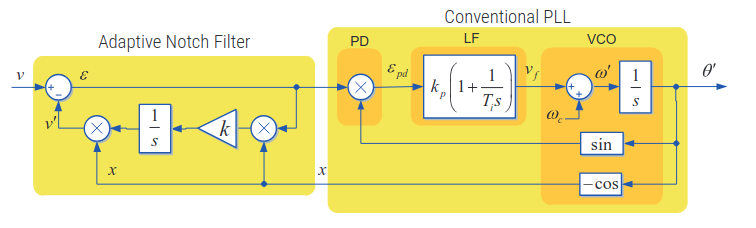
\includegraphics[width=0.8\linewidth]{IMAGES/Indus_el/Screenshot from 2024-11-18 08-26-49.png}
\end{figure}

ANC output is zero only if frequency and phase angle of $v$ and $x$ match. If interested only in frequency, we need to remove phase angle dependency.\\
The adaptive filter TF is then : $AF(s) = \frac{s}{s^2 + \omega^{'2}} = \frac{v'}{g}$ with $g(s) = k \varepsilon_v$. This TF is a Generalized Integrator.\\
\begin{itemize}
    \item Adaptive Band-pass Filter : $ABPF(s) = \frac{v'(s)}{v(s)} = \frac{ks}{s^2 + ks+\omega^{'2}}$
    \item Adaptive Notch Filter : $ANF(s) = \frac{\varepsilon(s)}{v(s)} = \frac{s^2 + \omega^{'2}}{s^2 + ks + \omega^{'2}}$
    \item Adaptive Low-pass filter : $ALPF(s) = \frac{qv'(s)}{v(s)} = \frac{k \omega^{'2}}{s^2 + ks + \omega^{'2}}$
\end{itemize}

\begin{figure}[hbt!]
    \centering
    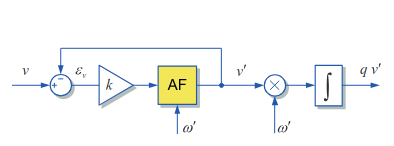
\includegraphics[width=0.5\linewidth]{IMAGES/Indus_el/Screenshot from 2024-11-18 08-37-34.png}
    \caption{QSG based on 2nd order AF}
\end{figure}

\warning Our performance depends on the gain and frequency which is not so good.\\
Then, we can develop a Second Order Generalized integrator (SOGI) : \\

Input $\omega'$ to the GI instead of $\omega^{'2}$.\\

\begin{itemize}
    \item $SOGI(s) = \frac{v'(s)}{k \varepsilon_v} = \frac{\omega's}{s^2+\omega^{'2}}$
    \item $D(s) = \frac{v'(s)}{v(s)} = \frac{k \omega's}{s^2 + k \omega's + \omega^{'2}}$
    \item $Q(s) = \frac{qv'(s)}{v(s)} = \frac{k\omega^{'2}}{s^2 + k \omega's + \omega^{'2}}$
\end{itemize}
With : \begin{itemize}
    \item $\tau = \frac{2}{k\omega'}$
    \item $t_s = 4.6 \tau$
    \item $k = \frac{9.2}{t_s \omega'}$
\end{itemize}

\quad \underline{SOGI-PLL :}\\

\begin{figure}[hbt!]
    \centering
    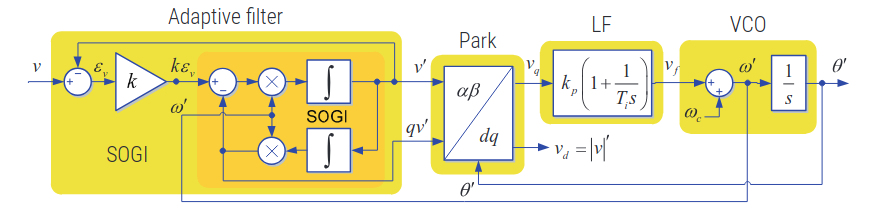
\includegraphics[width=0.8\linewidth]{IMAGES/Indus_el/Screenshot from 2024-11-18 08-53-37.png}
\end{figure}

SOGI-QSG can be used to implement PLL based on in-quadrature signal generation. We have noise canceling/harmonic filtering and fast transient response.\\

The SOGI could also be applied to FLL.\\

\subsubsection{Unbalanced grid conditions}
We can use Fortescue Symmetrical Components : $\begin{pmatrix}
    v^+\\ v^- \\ v^0
\end{pmatrix} = \frac{1}{3} \begin{pmatrix}
    1 & \alpha & \alpha^2\\
    1 & \alpha^2 & \alpha\\
    1 & 1 & 1\\
\end{pmatrix} \begin{pmatrix}
    v_a\\ v_b\\ v_c
\end{pmatrix}$, with $\alpha = e^{j2\pi/3}$ and $v_x$ are phasors.\\
Then $v_{abc} = v_{abc}^n + v_{abc}^{-n} + v_{abc}^{0n}$.\\
In general, positive-sequence voltage vector at fundamental frequency interacts with positive or negative sequence nth-order harmonic.\\
Then, in the dq frame, we might have $v_{dq} = \frac{3}{2} V^{+1} \begin{pmatrix}
    1\\0
\end{pmatrix} + \frac{3}{2} V^n \begin{pmatrix}
    \cos((n-1) \omega t)\\
    \sin((n-1) \omega t)
\end{pmatrix}$\\
\begin{itemize}
    \item module $\lvert v_{dq} \rvert$ is not constant
    \item phase angle $\theta$ is not constant
\end{itemize}

Then, we can develop the DSRF method : two frames of reference dq : $dq^{1}$ rotating with speed $\omega'$ and $dq^{-1}$ rotating with speed $-\omega'$.\\
Then, we have : \begin{itemize}
    \item $v_{dq}^1 = V^{+1} \begin{pmatrix}
        1 \\ 0
    \end{pmatrix} + V^{-1} \begin{pmatrix}
        \cos(-2\omega t)\\ \sin(-2\omega t)
    \end{pmatrix}$
    \item $v_{dq}^{-1} = V^{-1} \begin{pmatrix}
        1 \\ 0
    \end{pmatrix} + V^{+1} \begin{pmatrix}
        \cos(2\omega t)\\ \sin(2\omega t)
    \end{pmatrix}$
\end{itemize}

There is a second harmonic ripple. In general it is a m harmonic ripple.\\

We need to decouple the network to get rid of this harmonic ripple (DDSRF).\\

\begin{figure}
    \centering
    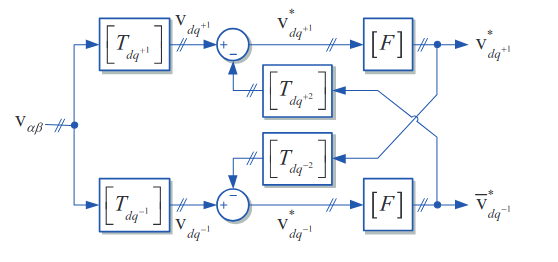
\includegraphics[width=0.8\linewidth]{IMAGES/Indus_el/Screenshot from 2024-11-18 09-23-18.png}
    \caption{DDSRF block diagram (for n=1, m=1)}
\end{figure}

In a stationary reference frame ($\alpha \beta$), we can apply Lyon transformation.\\



\subsection{MPPT PQ theory}

\subsubsection{MPPT}
Maximum power extraction from the renewable energy source.\\

\begin{figure}[hbt!]
    \centering
    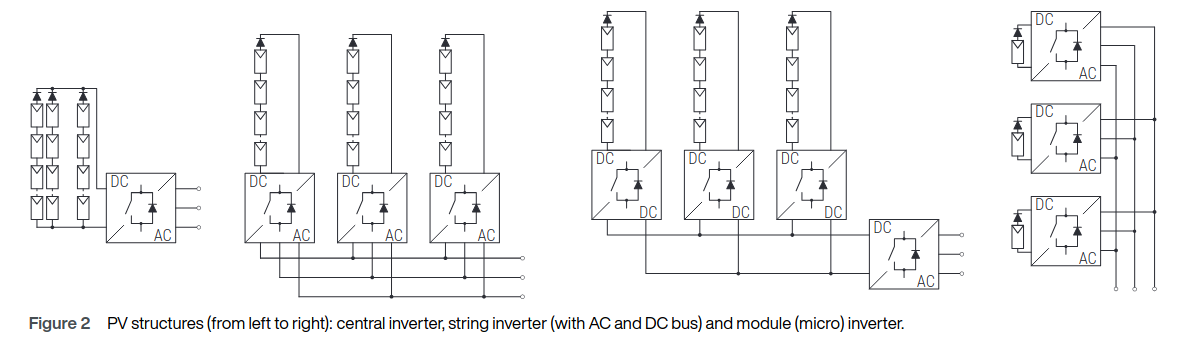
\includegraphics[width=0.8\linewidth]{IMAGES/Indus_el/Screenshot from 2024-11-11 08-41-35.png}
\end{figure}

\quad \underline{PV panel characteristics :}\\
PV panel output characteristics is influenced with : \begin{itemize}
    \item Irradiation : output current increases with higher irradiation
    \item Temperature : open circuit voltage increases with lower temperature
\end{itemize}
$v_{OC}$ : open circuit voltage, $i_{SC}$ : short circuit current\\

\begin{figure}[hbt!]
    \centering
    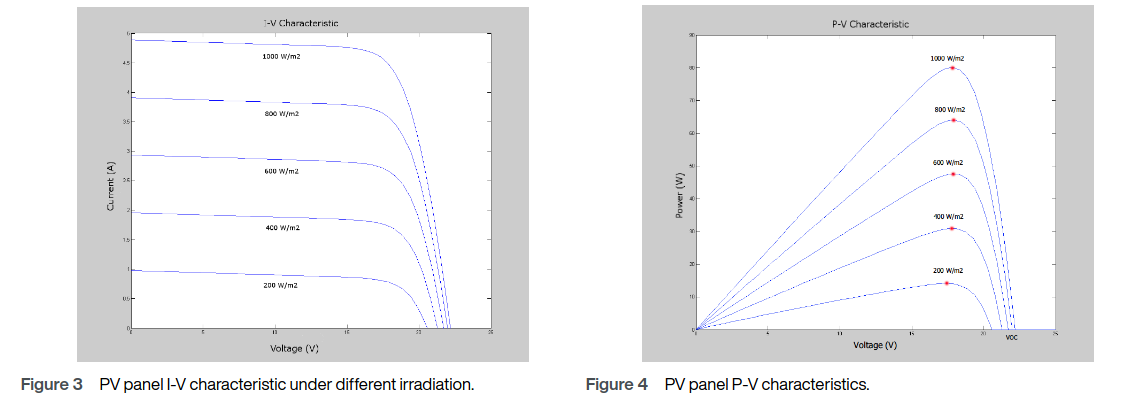
\includegraphics[width=0.8\linewidth]{IMAGES/Indus_el/Screenshot from 2024-11-11 08-45-37.png}
\end{figure}

\begin{figure}[hbt!]
    \centering
    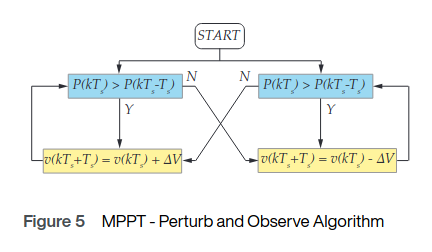
\includegraphics[width=0.5\linewidth]{IMAGES/Indus_el/Screenshot from 2024-11-11 08-49-55.png}
\end{figure}

Multiple sorts of algorithm can be implemented : \begin{itemize}
    \item Perturb and Observe : \begin{itemize}
        \item perturbation is introduced in the panel operating voltage $v_{PV}$
        \item power is then calculated and compared with before
        \item based on this, voltage $v_{PV}$ is adjusted
        \item decreasing voltage while on the right side of MMP increases output power
        \item once MPP is reached, it oscillates around this value
    \end{itemize}
    \item Incremental conductance : it uses the fact that the power curve derivative is zero at MPP ($\frac{d P_{PV}}{dv_{PV}} \Rightarrow \frac{\Delta i_{PV}}{ \Delta v_{PV}} = - \frac{i_{PV}}{v_{PV}}$). One here only has to compare the derivatives.
\end{itemize}

\subsubsection{Sequence decomposition}
To analyse unbalanced polyphase networks, we should use a method of symmetrical components. SS phasors of an unbalanced system can be decomposed into : \begin{itemize}
    \item Positive-sequence components
    \item Negative-sequence components
    \item Zero-sequence components
\end{itemize}

The different sequence phasors of phase a is : $V_{(a),-,+} = [T_{+,-,0}] V_{abc}$ with $T_{+,-,0} = \frac{1}{3} \begin{pmatrix}
    1 & \alpha & \alpha^2\\
    1 & \alpha^2 & \alpha\\
    1 & 1 & 1
\end{pmatrix}$

This method can be applied in the time domain. \\

\quad `\underline{Clarke transformation - Scaling :}\\
Depending on the objectives Clarke Transform scaling can be adjusted accordingly.
\begin{itemize}
    \item Power Invariant Form ($K = \sqrt{\frac{2}{3}}$) : amplitudes are not the same in the abc and $\alpha \beta 0$ frames
    \item Power non-invariant form ($K = \frac{2}{3}$) : amplitudes are the same in the abc and $\alpha \beta 0$ frames
\end{itemize}
\begin{equation}
    \begin{pmatrix}
        v_\alpha \\ v_\beta \\v_0
    \end{pmatrix} = K \begin{pmatrix}
        1 & -\frac{1}{2} & \frac{1}{2}\\
        0 & \frac{\sqrt{3}}{2} & -\frac{\sqrt{3}}{2}\\
        \frac{1}{\sqrt{2}} & \frac{1}{\sqrt{2}} & \frac{1}{\sqrt{2}}\\
    \end{pmatrix}
\end{equation}


\subsubsection{Instantaneous Power Theory}
For a given phase-to-neutral voltage and currents in abc domain, we can apply Clarke Transform : $v_{\alpha \beta 0} = [T_{\alpha \beta 0}] v_{abc}$ (same for $i$).\\
The instantaneous power are defined in the $\alpha \beta 0$ frame : $\begin{pmatrix}
    p_{\alpha \beta}\\ q_{\alpha \beta} \\ p_0\\
\end{pmatrix} = M_{\alpha \beta 0} i_{\alpha \beta 0}$ where $M_{\alpha \beta 0} = \begin{pmatrix}
    v_\alpha & v_\beta & 0 \\
    -v_\beta & v_\alpha & 0\\
    0 & 0 & v_0\\
\end{pmatrix}$
The instantaneous active power delivered collectively by 3-phases of a system is $p_{\alpha \beta} + p_0$.\\

It should be considered that $p$ and $q$ contain both constant and oscillatory components.\\

Power definitions are preserved with change of reference frame from $\alpha \beta$ to $dq$ : \begin{itemize}
    \item $p_{dq} = v_d i_d + v_q i_q$ - instantaneous real power
    \item $q_{dq} = v_d i_q - v_q i_d$ - instantaneous imaginary power
\end{itemize}
By orienting $dq$ frame in such a way that the d-axis is perfectly aligned with grid voltage space vectors ($v_q = 0$), we have : \begin{itemize}
    \item $p_{dq} = v_d i_d$
    \item $q_{dq} = v_d i_q$
\end{itemize}
These expressions assume Clarke scaling of $K = \sqrt{\frac{2}{3}}$ (For scaling of $K = \frac{2}{3}$, we have $p_{dq} = \frac{3}{2} (v_d i_d + v_q i_q)$ and $q_{dq} = \frac{3}{2} (v_d i_q - v_q i_d)$)\\

\subsection{LCL filter}
Power exchange between point A and B : $S = V_A I^* = \frac{V_A^2}{Z} \langle \theta - \frac{V_AV_B}{Z} \langle(\theta + \delta)$. $\delta$ is the power angle and $\theta$ the power factor angle. We have : $P_A = \frac{V_A}{R^2+X^2} [R(V_A-V_B \cos\delta) + XV_B \sin \delta]$ and $Q_A = \frac{V_A}{R^2+X^2} [-RV_B \sin \delta + X(V_a-V_B\cos\delta)]$. As $X>>R$ and $\delta<<1$ : $P_A = \frac{V_AV_B}{X} \delta$and $Q_A = \frac{V_A-V_B}{X}V_A$. One need to control the power angle to control the active power.\\

In case of low switching frequencies, LC trap filters are used : series connected LC elements are tuned to a specific resonance frequency, at series resonance frequency impedance of the filter is at minimum, this represents low impedance path for current harmonic at that frequency. Resonant frequency is calculated as : $f_r = \frac{1}{2\pi LC}$. (In practice, depending on the country there is a limit to the amount of harmonics you can bring into the grid)\\
Several series LC elements tuned at different frequencies can be connected in parallel (LC in series connected between the line and the ground). Impedance of LC circuit ignoring resistances is : $Z_{LC} = \frac{s^2 LC +1}{sC}$.

\begin{figure}[hbt!]
    \centering
    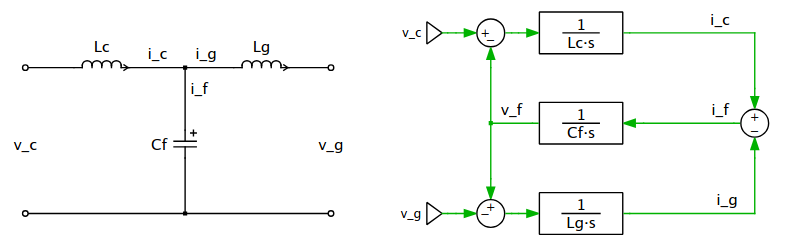
\includegraphics[width=0.5\linewidth]{IMAGES/Indus_el/Screenshot from 2024-11-25 08-28-33.png}
    \caption{Single-phase ideal LCL filter and model.}
\end{figure}

Resistances are neglected : $v_c(s) = sL_c i_c(s) + v_f(s)$, $v_g(s) = v_f(s) - sL_g i_g(s)$, $v_f(s) = \frac{i_f(s)}{sC_f}$, $i_c(s) = i_f(s) + i_g(s)$. The transfer function of $\frac{i_g(s)}{v_c(s)}$ with $v_g(s) = 0$ is then : \begin{equation}
    H_{LCL}(s) = \frac{1}{L_c C_f L_g s^3 + (L_c + L_g)s}
\end{equation}

The resonant frequency is then : $\omega_r = \sqrt{\frac{1}{L_{eq} C_f}}$ with $L_{eq} = \frac{L_cL_g}{L_c+L_g}$. The frequency response show high peak at resonant frequency and a $-60 dB$ attenuation slope at higher frequencies.\\
Certain limits : capacitor value is limited by decrease of power factor at rated power, total value of inductance should be less than 0.1pu to limit AC voltage drop, the resonant frequency should be in the range between tens times the grid frequency and one half the switching frequency. \\

\subsubsection{Design}
\quad \underline{C :}\\
Filter capacitance is related to the base value as percentage of it : $C_f = x C_b$ (usually $x \in [1-5]\%$). With : $Z_b = \frac{V_{LL}^2}{P_n}$, $C_b = \frac{1}{\omega_b Z_b}$, $L_b = \frac{Z_b}{\omega_g}$.\\

\quad \underline{$L_c$ :}\\
We assume short circuit conditions for $C_f$ at ripple frequency. The maximum current ripple ot the output of a 3-phase 2-level VSI can be determined as : $\Delta i_{Lc, max} = \frac{V_{DC}}{6L_c f_{sw}}$. Then, one has to choose the desired current ripple (here $10\%$) : $\Delta i_{Lc,max} = 0.1 I_{Lc,peak}$.\\
With $I_{Lc,max} = \frac{P_n}{\sqrt{3} V_{LL}} \Rightarrow I_{Lc,peak} = \sqrt{2} I_{Lc,max}$. Then, the minimum inductance is value : $L_{c,min} = \frac{V_{DC}}{6 \Delta i_{Lc,max} f_{sw}}$ and $L_c = rL_g$ with r a scaling factor.\\

\quad \underline{$L_g$ :}\\
One has to consider harmonic attenuation, resonant frequency. Neglecting losses, grid current harmonic attenuation can be defined as : $\frac{i_g(h_{sw})}{i_c(h_{sw})} = \frac{1}{\lvert 1+ r(1-L_g x C_b \omega_{sw}^2)\rvert} = k_a$ with $L_c$ already selected and $k_a$ represents the desired attenuation at switching frequency.\begin{equation}
    L_g = \frac{\sqrt{\frac{1}{k_a^2}} +1}{C_f \omega_{sw}^2}
\end{equation}

One could choose $L_c = L_g$ as it provides good compromise. In practice, grid inductance is part of $L_g$.\\

\subsubsection{Passive damping}
Zero impedance at the LCL filter resonant frequency may lead to control instability. One can add a resistor in series with the capacitor. The TF linking filter output $i_g$ with filter input $v_c$ is : $H_{LCL}(s) = \frac{C_f R_f s +1}{L_c C_f L_g s^3 + C_f (L_c+L_g) R_f s^2 + (L_c+L_g)s}$. Damping resistance attenuates the high peak gain but reduces filter effectiveness and increases losses. Usually : \begin{equation}
    R_f = \frac{1}{3\omega_{res} C_f}
\end{equation}

\subsubsection{Active damping}
Rather than using passive damping with a real resistor, it is possible to achieve similar effect by means of control and virtual resistor.\\
Let $v_f$ be the capacitor voltage and $i_f$ the capacitor voltage. The two TF of interest : \begin{equation}
    \begin{gathered}
        H^d_{v_f}(s) = \frac{v_f(s)}{v_c(s)} = \frac{1+s R_f C_f}{L_c C_f} \frac{1}{s^2 + \omega_r^2(1+s R_f C_f)}\\
        H^d_{i_f}(s) = \frac{i_f(s)}{v_c(s)} = \frac{1}{L_c} \frac{s}{s^2 + \omega_r^2(1+sR_fC_f)}\\
    \end{gathered}
\end{equation}
Ideally, we would like to achieve $H_{v_f}^d(s)$ without real $R_f$ but with $R_v$ (virtual). Let's call $H_{v_f}(s) = H_1(s)$ (without any $R_f$) and $H_{v_f}^d(s) = H_3(s)$.\\
Then, the closed loop TF of the controller : $H_{CL}(s) = \frac{H_1(s)}{1+H_1(s) H_2(s) K_{AD}}$ with $K_{AD} = \frac{L_c+L_g}{L_g} R_v$. We have : $H_{CL}(s) = \frac{L_g}{s^2 L_c C_f L_g + (L_c+L_g)(1+sR_v C_f)}$.\\
Implementation must consider both axis of regulator ($v_q$, $v_d$).\\
With the d-axis perfectly aligned with grid voltage ($v_g=0$), we have $p_d = \frac{3}{2} v_d i_d$ and $p_q = -\frac{3}{2}v_di_q$. \\
Equivalent impedance at the PCC (point of common coupling) will depend on position of voltage and current sensor : \begin{itemize}
    \item $V_f$ and $i_c$ sensed : $Z_g = R+j(X_2+X_g-X_c)$, $Z_c=R+jX_1$
    \item $V_f$ and $i_g$ sensed : $Z_g = R+j(X_2+X_g)$, $Z_c=R+j(X_1-X_c)$
    \item $\cdots$
\end{itemize}

\subsection{Small signal dynamic modeling}
We can consider two generic cases of Grid Connected 2L-3phase converter (VSI) : Current Fed VSI (some other input converter behaves as current source), Voltage Fed VSI (some other input converter manages DC-link voltage).\\



\end{document}